%=======================================================
%	PACKAGES AND THEMES
%=======================================================
\documentclass[8pt]{beamer}
\mode<presentation> {
\usepackage{etex}
\usetheme{Boadilla}
\definecolor{navyblue}{rgb}{0.0, 0.0, 0.5}
\definecolor{dkgreen}{rgb}{0,0.6,0}
\definecolor{gray}{RGB}{64, 64, 64}
\definecolor{teal}{RGB}{0, 102, 102}
\definecolor{mauve}{rgb}{0.58,0,0.82}
\usecolortheme[named = navyblue]{structure}
\setbeamercolor{normal text}{fg = gray}
\setbeamercolor{frametitle}{fg = white, bg = navyblue}
\setbeamerfont{framesubtitle}{size = \normalsize}
\setbeamerfont{caption}{size=\footnotesize}
\setbeamercolor{page number in head/foot}{fg = gray}
\setbeamertemplate{footline}%[frame number]
}


\usepackage{graphicx} % Allows including images
\usepackage{booktabs} % Allows the use of \toprule, \midrule and \bottomrule in tables
\usepackage{multicol}
\usepackage[export]{adjustbox}
\usepackage{colortbl}
\usepackage{graphicx} 

\usepackage{tikz}
\usepackage{fancybox}
\usepackage[absolute, overlay]{textpos}
\usepackage{multirow}
\usepackage{siunitx}
\usepackage{tcolorbox}


\usepackage{tikz}
\usepackage{calc}
\newlength{\outerradius}
\newlength{\innerradius}
\setlength{\outerradius}{0.50cm}
\setlength{\innerradius}{0.35cm}

%Damit wir Quellcode nutzen können.
\usepackage{listings}
\lstset{numbers=left,
	numberstyle=\tiny,
	numbersep=5pt,
	breaklines=true,
	showstringspaces=false,
	frame=l ,
	xleftmargin=15pt,
	xrightmargin=15pt,
	basicstyle=\ttfamily\scriptsize,
	stepnumber=1,
	keywordstyle=\color{blue},          % keyword style
  	commentstyle=\color{dkgreen},       % comment style
  	stringstyle=\color{mauve}         % string literal style
}
%Sprache Festelegen
\lstset{language=R}


%=======================================================
%	TITLE PAGE
%=======================================================

\title{\textbf{Principles of Infographics}\\
	      {\color{teal}{--Seminar--}}}

\author{Yasemin Aslan)}

\institute
{
SPRU (Science Policy Research Unit) \\
Business School\\
University of Sussex \\

\medskip

\medskip

\medskip

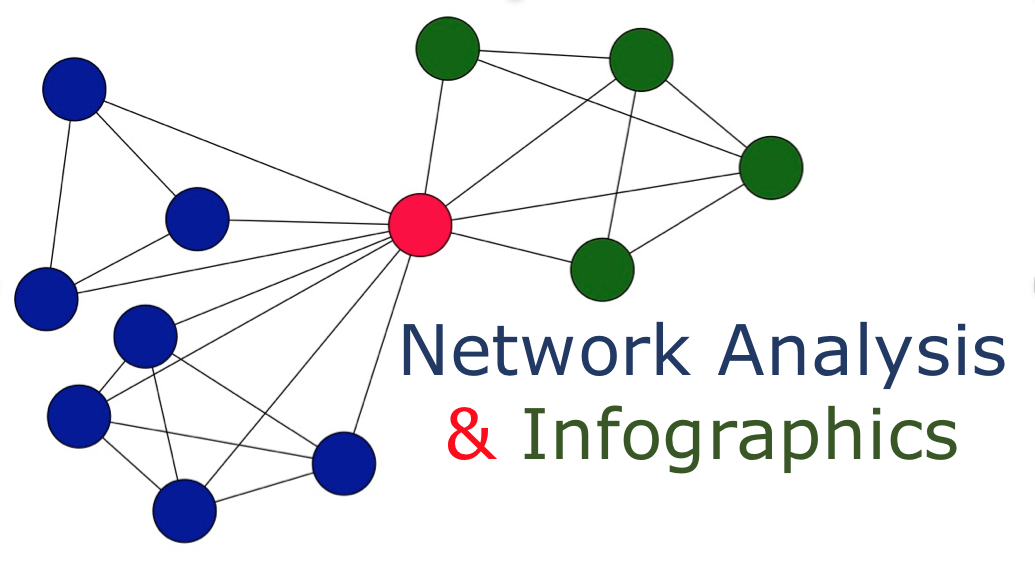
\includegraphics[width=2.5cm]{../_shared_pics/logo}

\medskip

\textit{{\color{dkgreen}{Week 7: 11 March 2022}}}\\
}


\date{} % Date, can be changed to a custom date

\begin{document}

\begin{frame}
\titlepage % Print the title page as the first slide

\begin{textblock*}{10pt}(0pt, 0.9\textheight)

\includegraphics[width=4cm]{../_shared_pics/SPRU.png}
\end{textblock*}

\end{frame}


%=======================================================
%	Learning outcomes
%=======================================================


\begin{frame}
\frametitle{\insertsection}
\framesubtitle{Learning Outcomes}

\centering
\begin{tabular}{lp{5.5cm}l}
\toprule
\multicolumn{2}{l}{\textbf{Learning outcome}} & \textbf{Assessment mode}\\
\hline
\\
1 & 
Explain the concept of network and list the main network indicators & 
ESS\\
\\
2 &  
Describe and apply the major techniques for the collection of network data and their statistical analysis & 
ESS, GPN + GWS\\
\\
3 & 
Identify the main characteristics of networks by means of network measures  & 
ESS, GPN + GWS\\
\\
\rowcolor{green!20}4 &
Employ network analysis techniques to produce network data-based infographics & 
GPN + GWS\\
\\
\bottomrule
\multicolumn{3}{l}{\scriptsize Note: ESS: Essay; GPN: Group Presentation; GWS: Group Written Submission}\\
\end{tabular}

\end{frame}

%------------------------------------------------


%=======================================================
%	Intro slides
%=======================================================

\begin{frame}
\frametitle{Overview}
\tableofcontents[hideallsubsections]
\end{frame}



%=======================================================
%	Network visualisation [recap]
%=======================================================
\section{Network visualisation [recap]}
%------------------------------------------------

\bgroup
\setbeamercolor{background canvas}{bg = navyblue}
\begin{frame}[plain]{}
\begin{center}
\color{white}{\Huge\insertsection}
\end{center}
\end{frame}
\egroup

%------------------------------------------------

\begin{frame}
\frametitle{\insertsection}
\framesubtitle{Layout}

Let's generate a network $G(N, E)$ where:
\begin{itemize}
\item $N=100$
\item $x_{ij} = 1$ with $p=0.02$
\end{itemize}
 
\end{frame}

%------------------------------------------------

\begin{frame}
\frametitle{\insertsection}
\framesubtitle{Layout: Random}

\centering
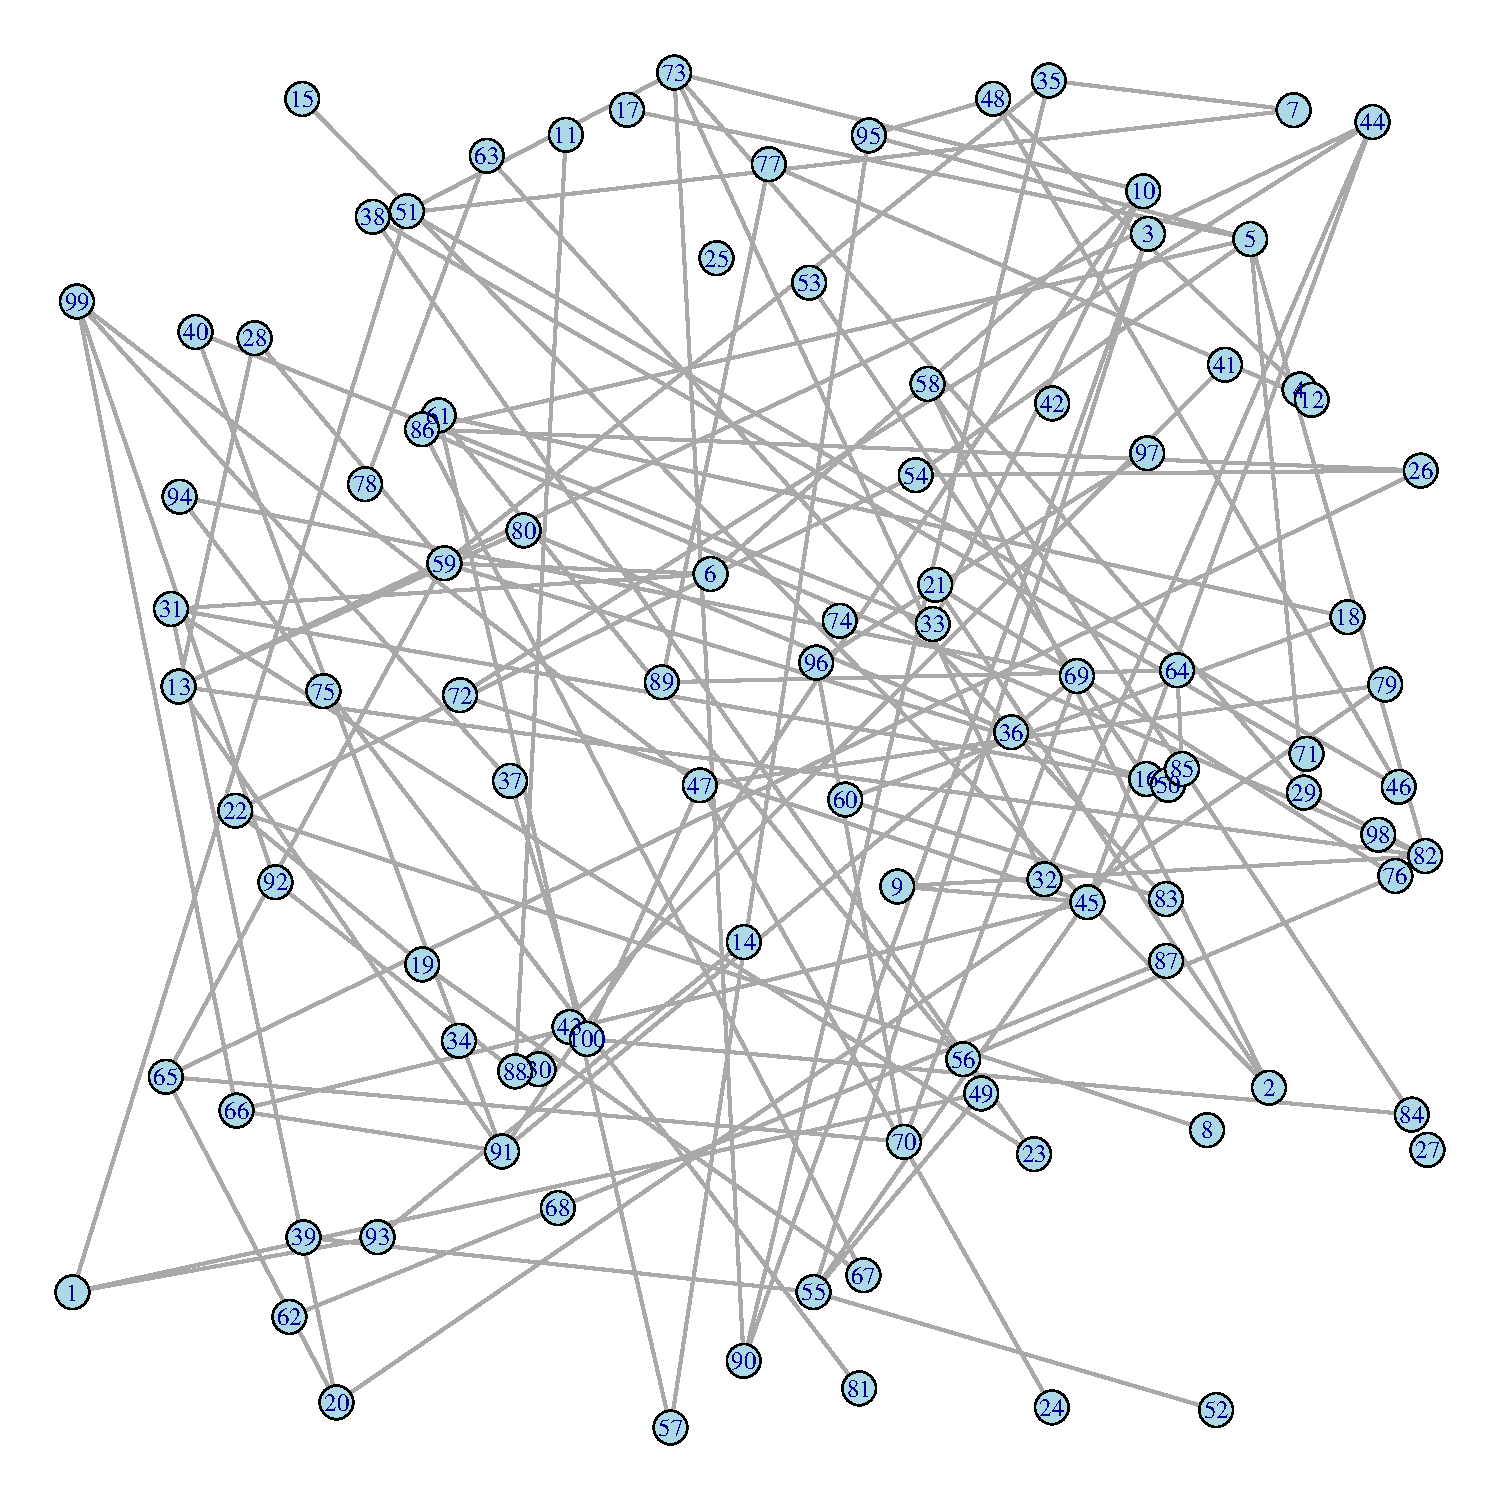
\includegraphics[height=0.85\textheight]{random}

\end{frame}

%------------------------------------------------

\begin{frame}
\frametitle{\insertsection}
\framesubtitle{Layout: Circle}

\centering
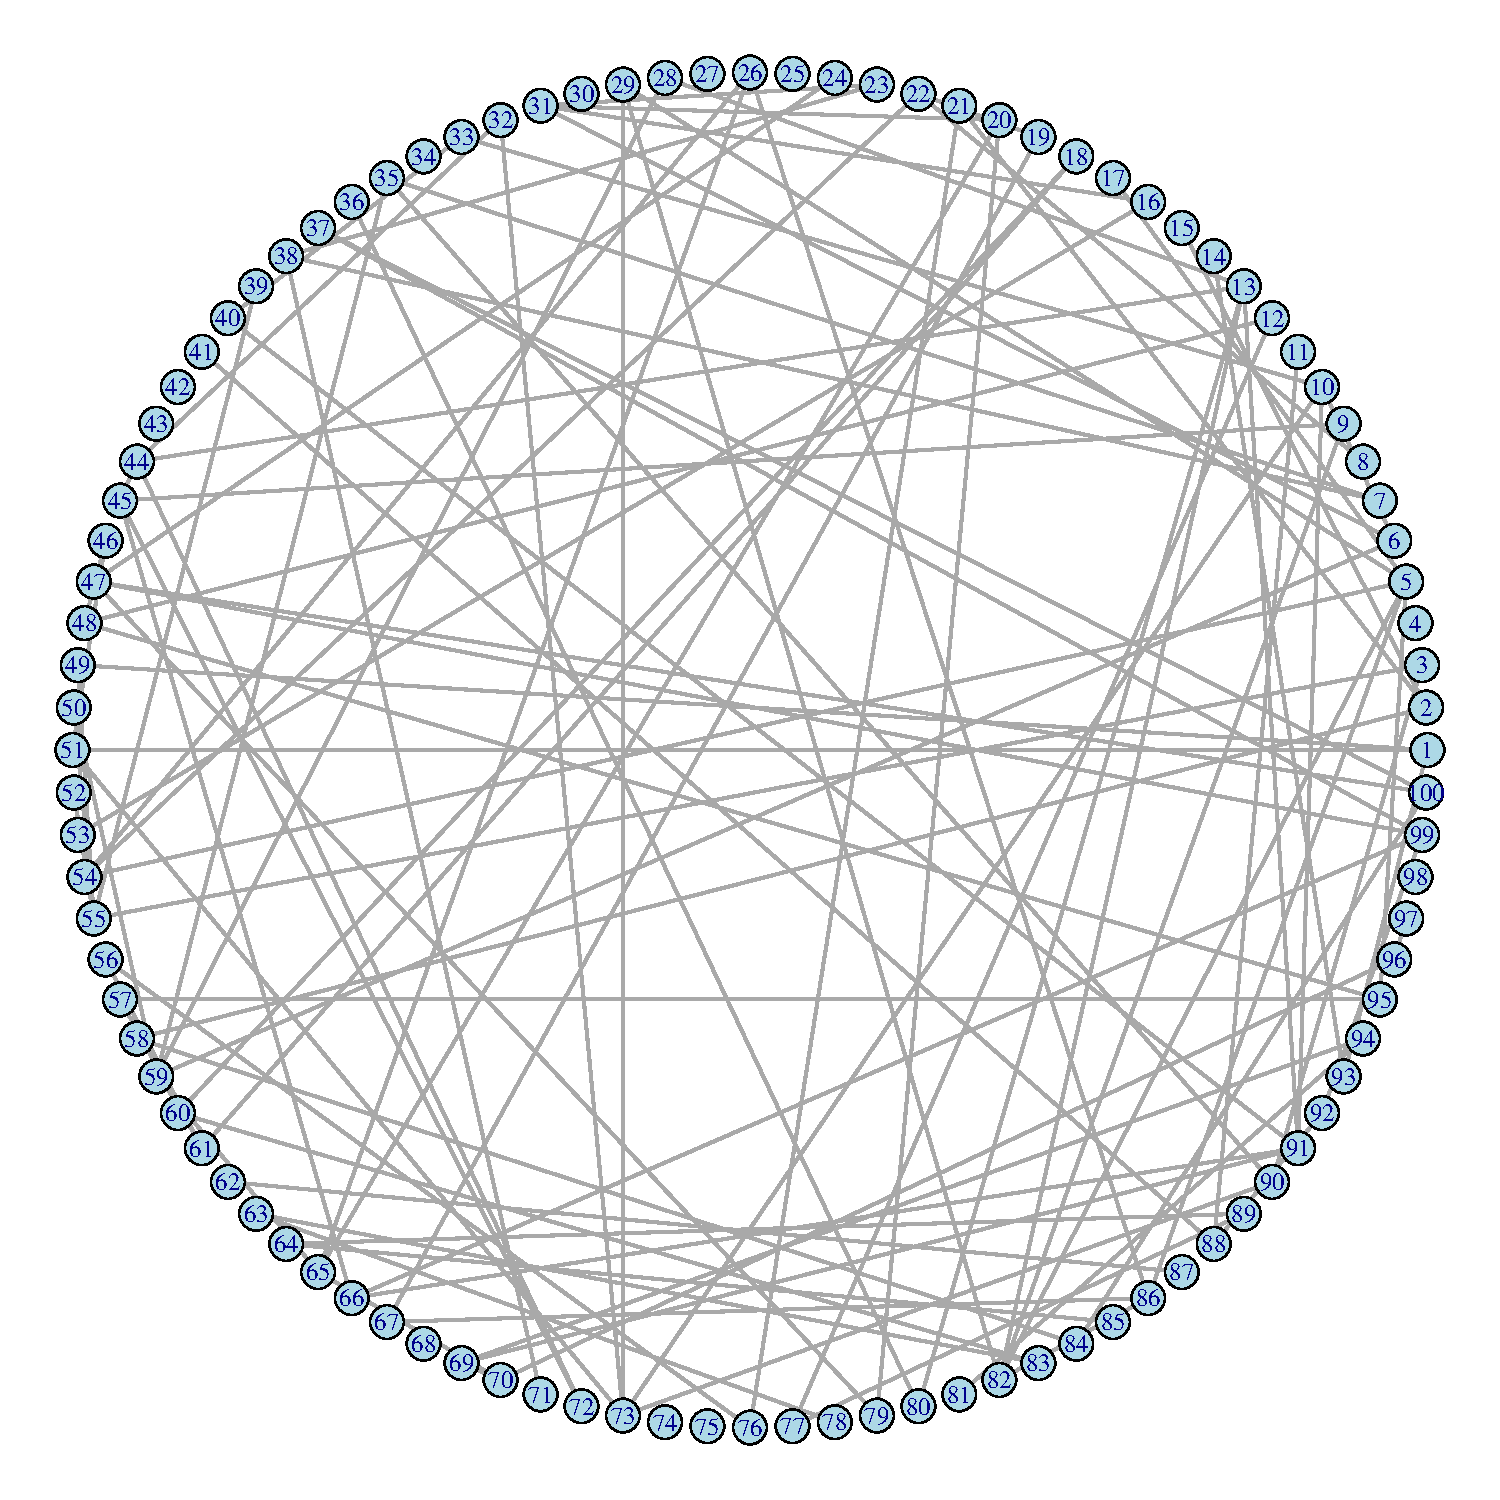
\includegraphics[height=0.85\textheight]{circle}

\end{frame}

%------------------------------------------------

\begin{frame}
\frametitle{\insertsection}
\framesubtitle{Layout: Grid}

\centering
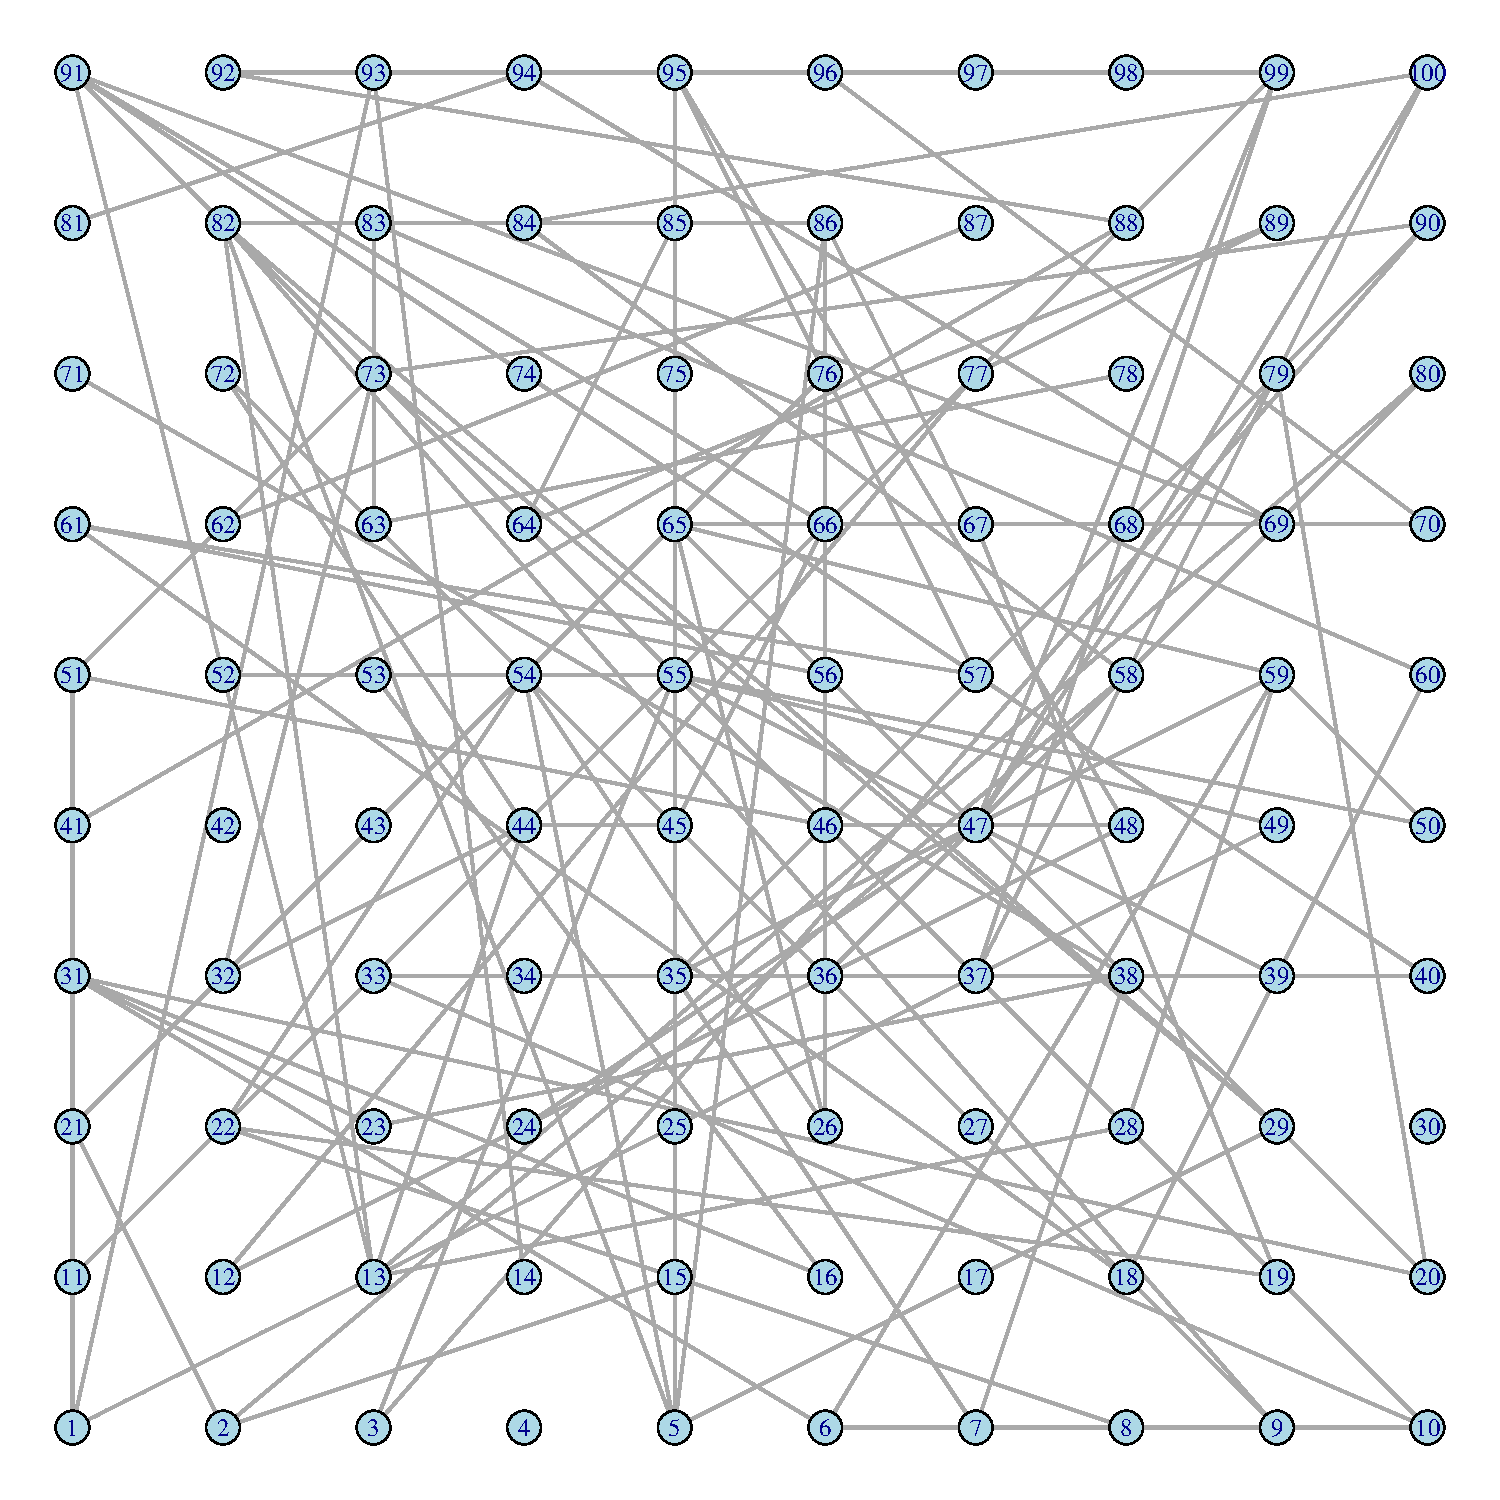
\includegraphics[height=0.85\textheight]{grid}
 
\end{frame}
%------------------------------------------------

\begin{frame}
\frametitle{\insertsection}
\framesubtitle{Layout: Kamada-Kawai}

\centering
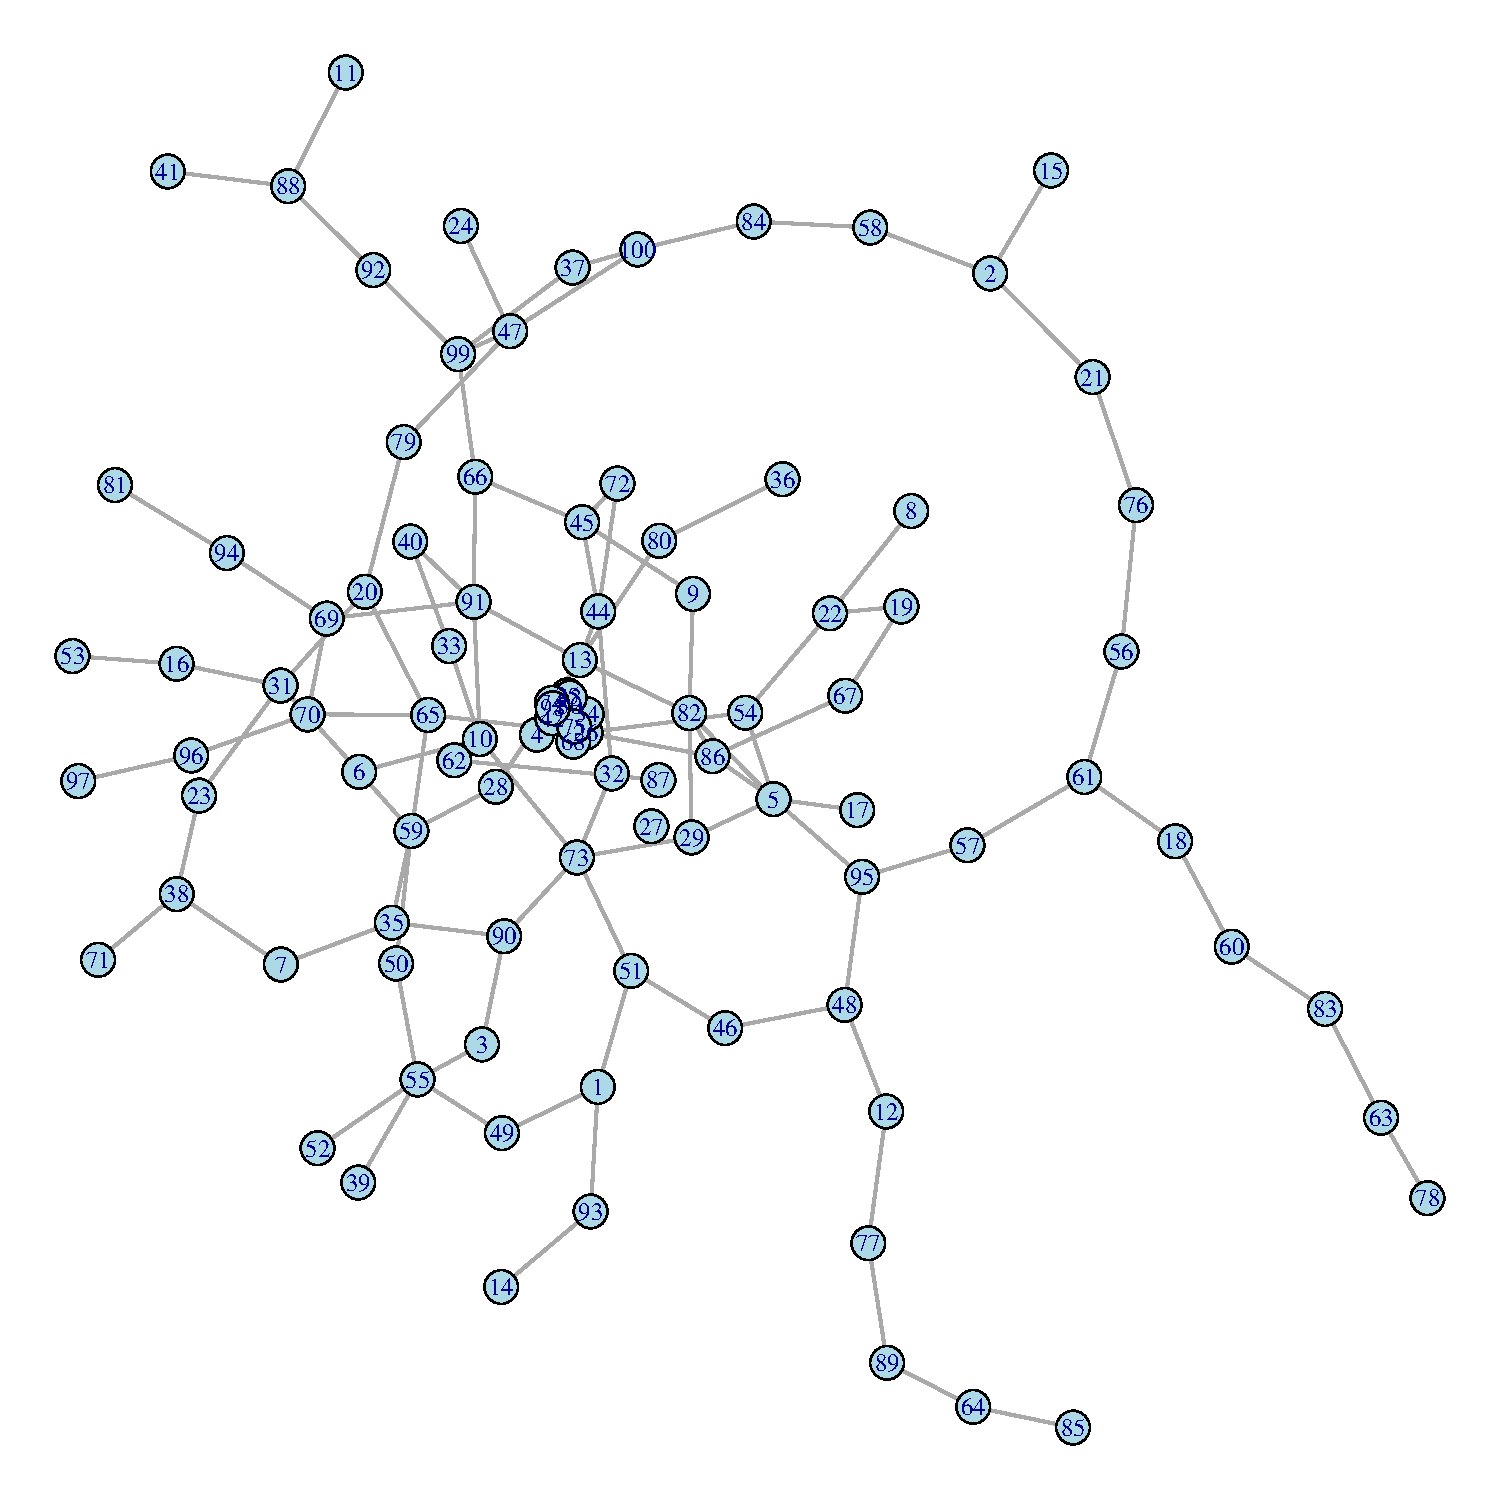
\includegraphics[height=0.85\textheight]{kamada}
 
\end{frame}

%------------------------------------------------

\begin{frame}
\frametitle{\insertsection}
\framesubtitle{Layout: Fruchterman and Reingold}

\centering
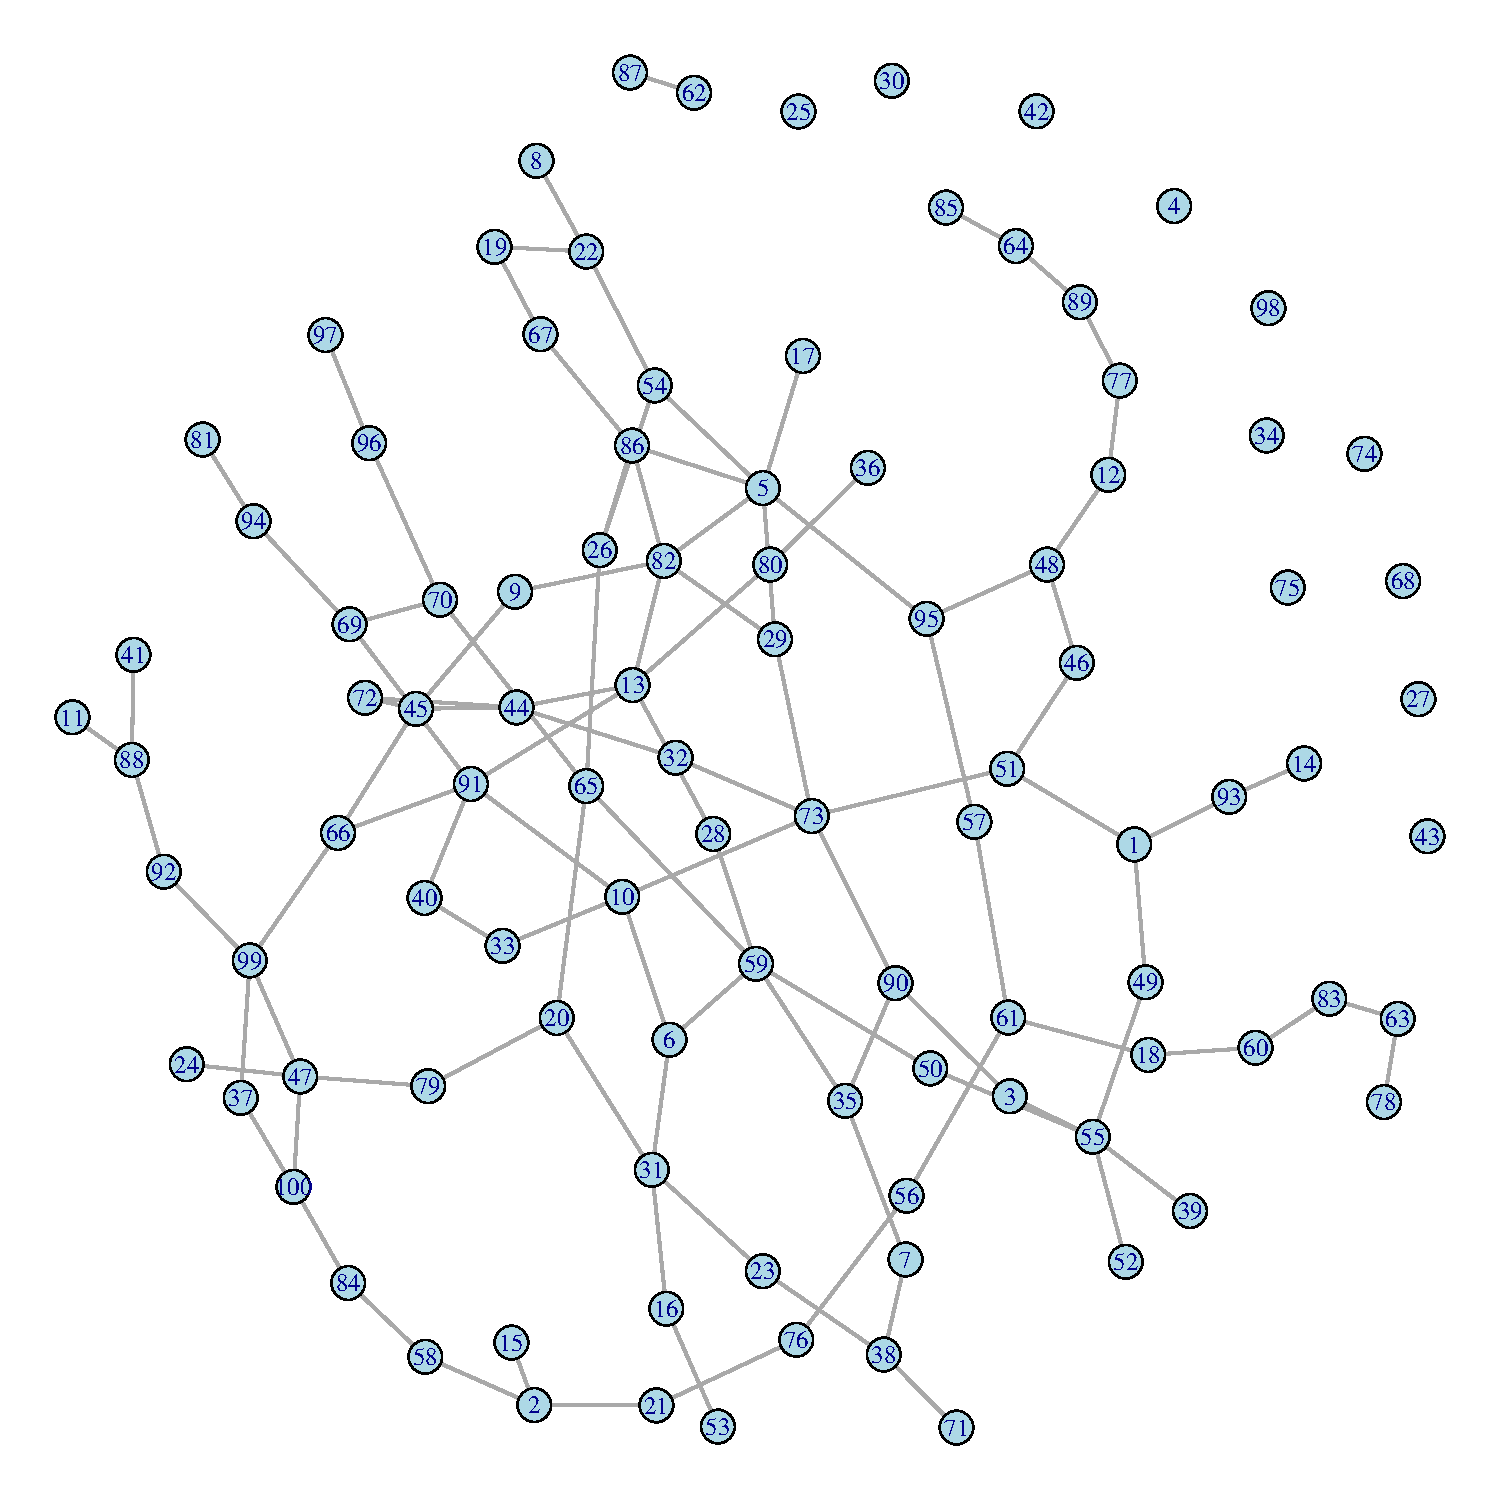
\includegraphics[height=0.85\textheight]{fr}
 
\end{frame}

%------------------------------------------------

\begin{frame}
\frametitle{\insertsection}

Let's practice this in RStudio (open S7\_Script.R)

\end{frame}

%------------------------------------------------
 


%=======================================================
% Introduction to Gephi
%=======================================================
\section{Introduction to Gephi}
%------------------------------------------------

\bgroup
\setbeamercolor{background canvas}{bg = navyblue}
\begin{frame}[plain]{}
\begin{center}
\color{white}{\Huge\insertsection}
\end{center}
\end{frame}
\egroup

%------------------------------------------------

\begin{frame}
\frametitle{\insertsection}

\begin{center}

\includegraphics[height=1.5cm]{gephi_logo}\\
\url{https://gephi.org/}
\end{center}

\begin{itemize}
\item Developed by the {\color{blue}{Gephi Consortium}} (a not-for-profit organisation)
\item Runs on {\color{blue}{Windows}}, {\color{blue}{Linux}}, {\color{blue}{Mac OSX}}
\item Relatively {\color{blue}{user-friendly}}
\item Can produce excellent {\color{blue}{network visualizations}}
\item Can read several {\color{blue}{file formats}}
\item Capable of analysing {\color{blue}{relatively large networks}}
\item Gephi plugins (\url{https://gephi.org/plugins})
\item Operation cannot be {\color{red}{automated}}
\end{itemize}

\end{frame}
%------------------------------------------------

\begin{frame}
\frametitle{\insertsection}
\framesubtitle{Interfaces}

\begin{itemize}
\item {\color{blue}{Overview}} 
    \begin{itemize}
    \item to generate network layouts
    \item to colour nodes/edge
    \item to calculate network measures
    \end{itemize}


\item {\color{blue}{Data laboratory}}
    \begin{itemize}
    \item to upload network data
    \item to manipulate network data
    \item to export network data
    \end{itemize}
    
    
\item {\color{blue}{Preview}}
    \begin{itemize}
    \item to preview network images
    \item to generate network images (e.g.\ pdf, jpeg)
    \end{itemize}

\end{itemize}

\end{frame}

%------------------------------------------------

\begin{frame}
\frametitle{\insertsection}
\framesubtitle{Overview interface}


\includegraphics[height=0.5cm]{gephi_logo}\\
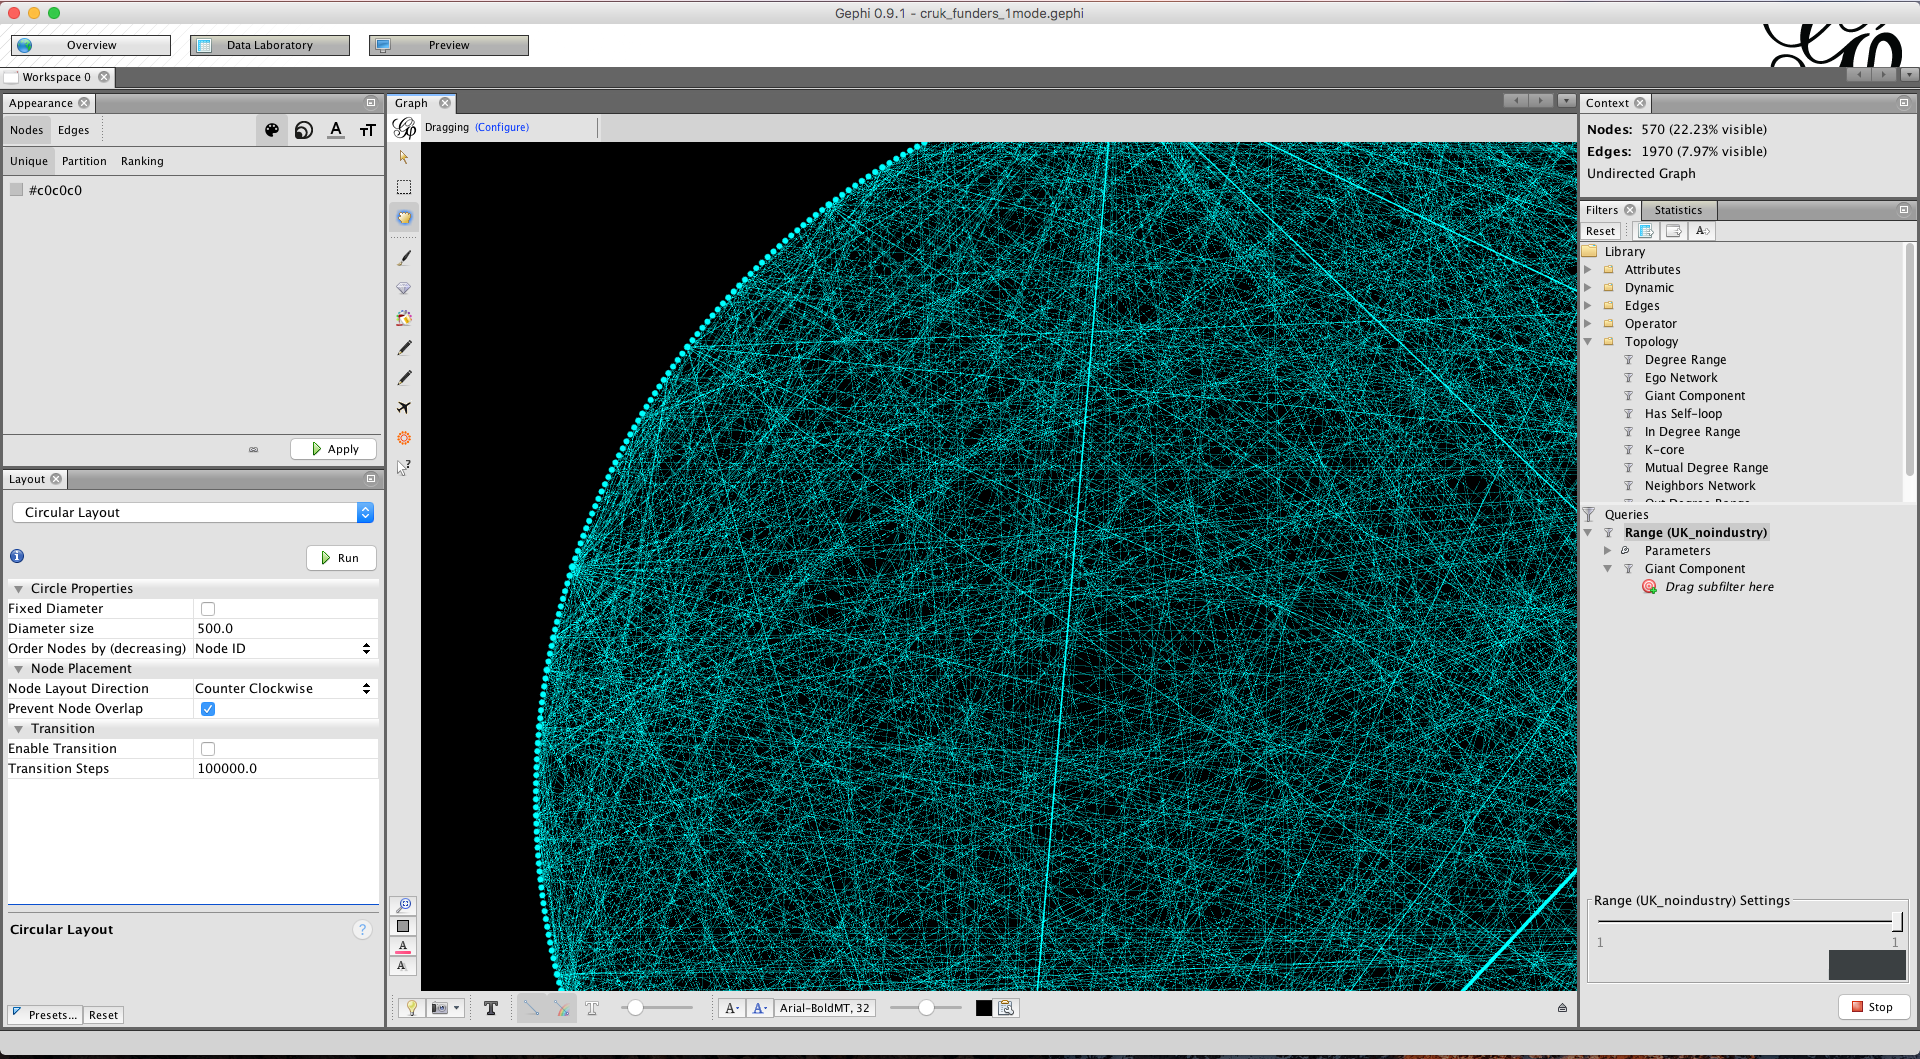
\includegraphics[width=\linewidth, frame]{gephi_interface1}

\end{frame}

%------------------------------------------------

\begin{frame}
\frametitle{\insertsection}
\framesubtitle{Data laboratory interface}


\includegraphics[height=0.5cm]{gephi_logo}\\
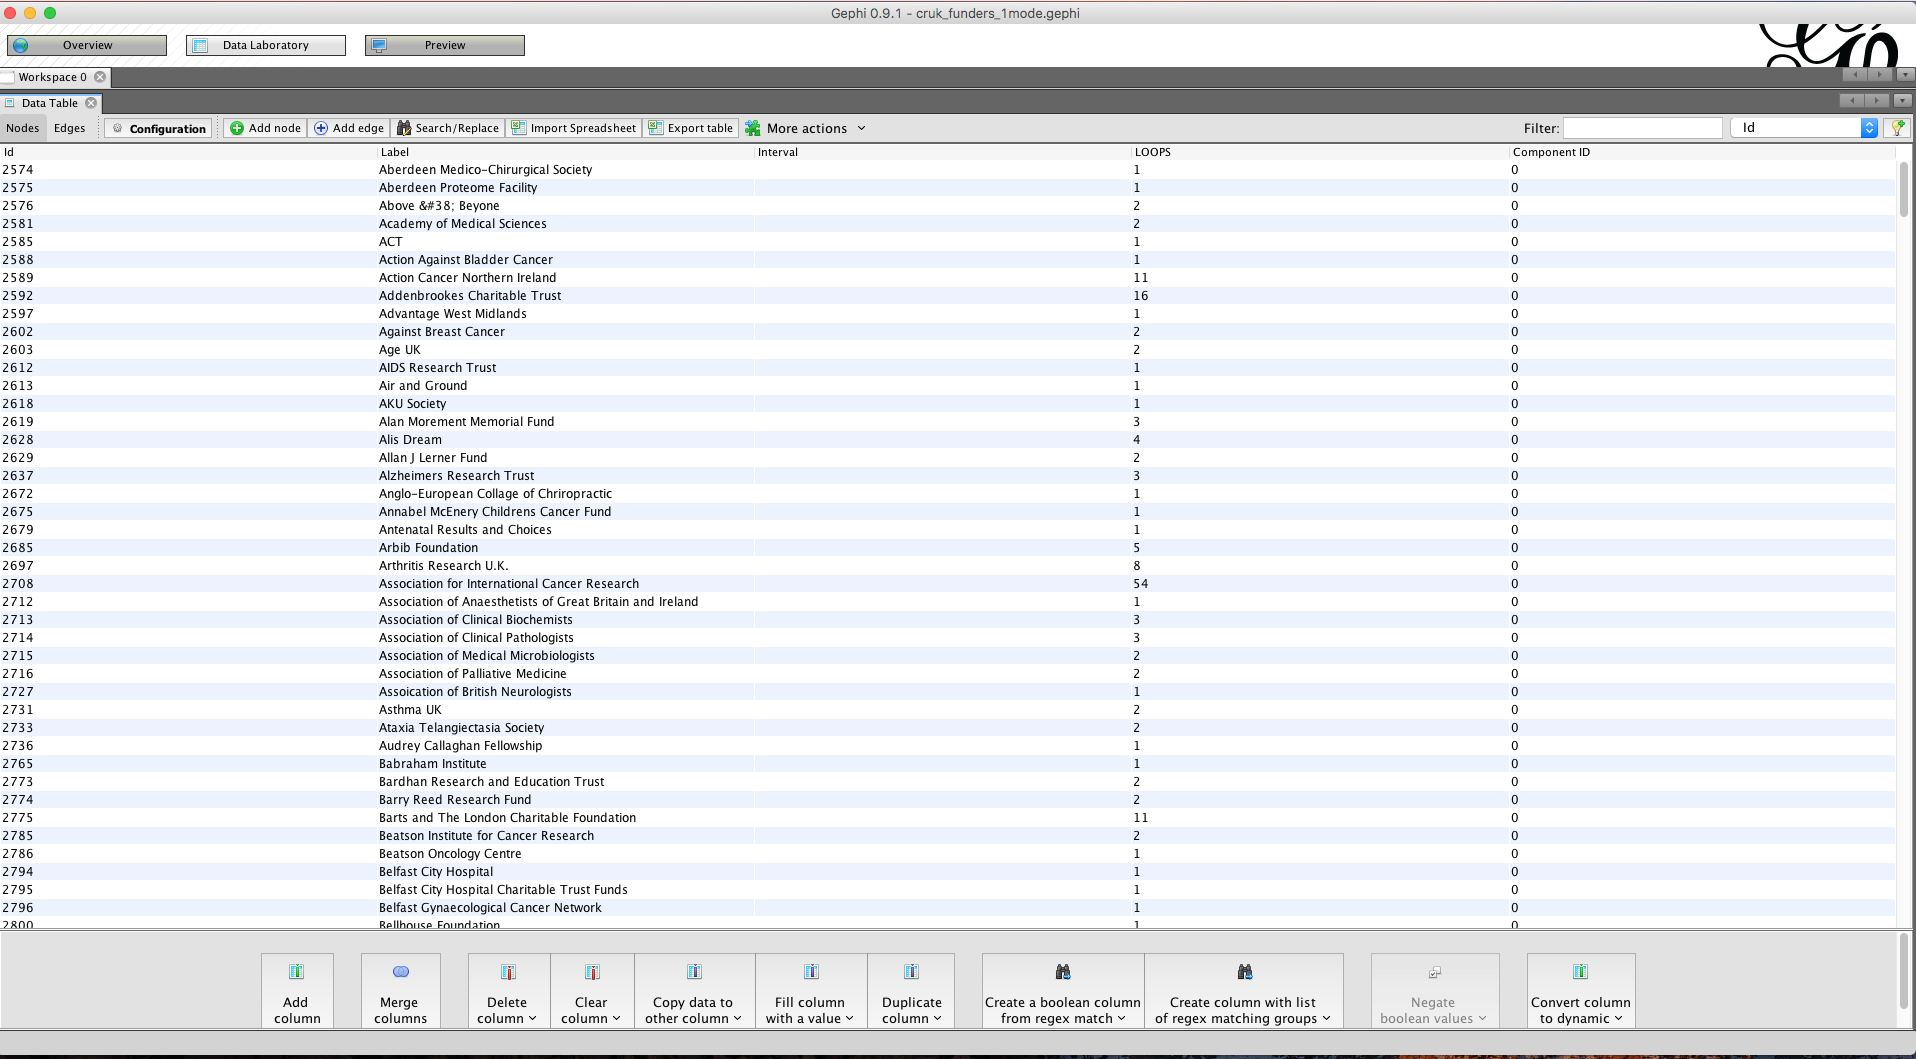
\includegraphics[width=\linewidth, frame]{gephi_interface2}

\end{frame}

%------------------------------------------------

\begin{frame}
\frametitle{\insertsection}
\framesubtitle{Preview interface}


\includegraphics[height=0.5cm]{gephi_logo}\\
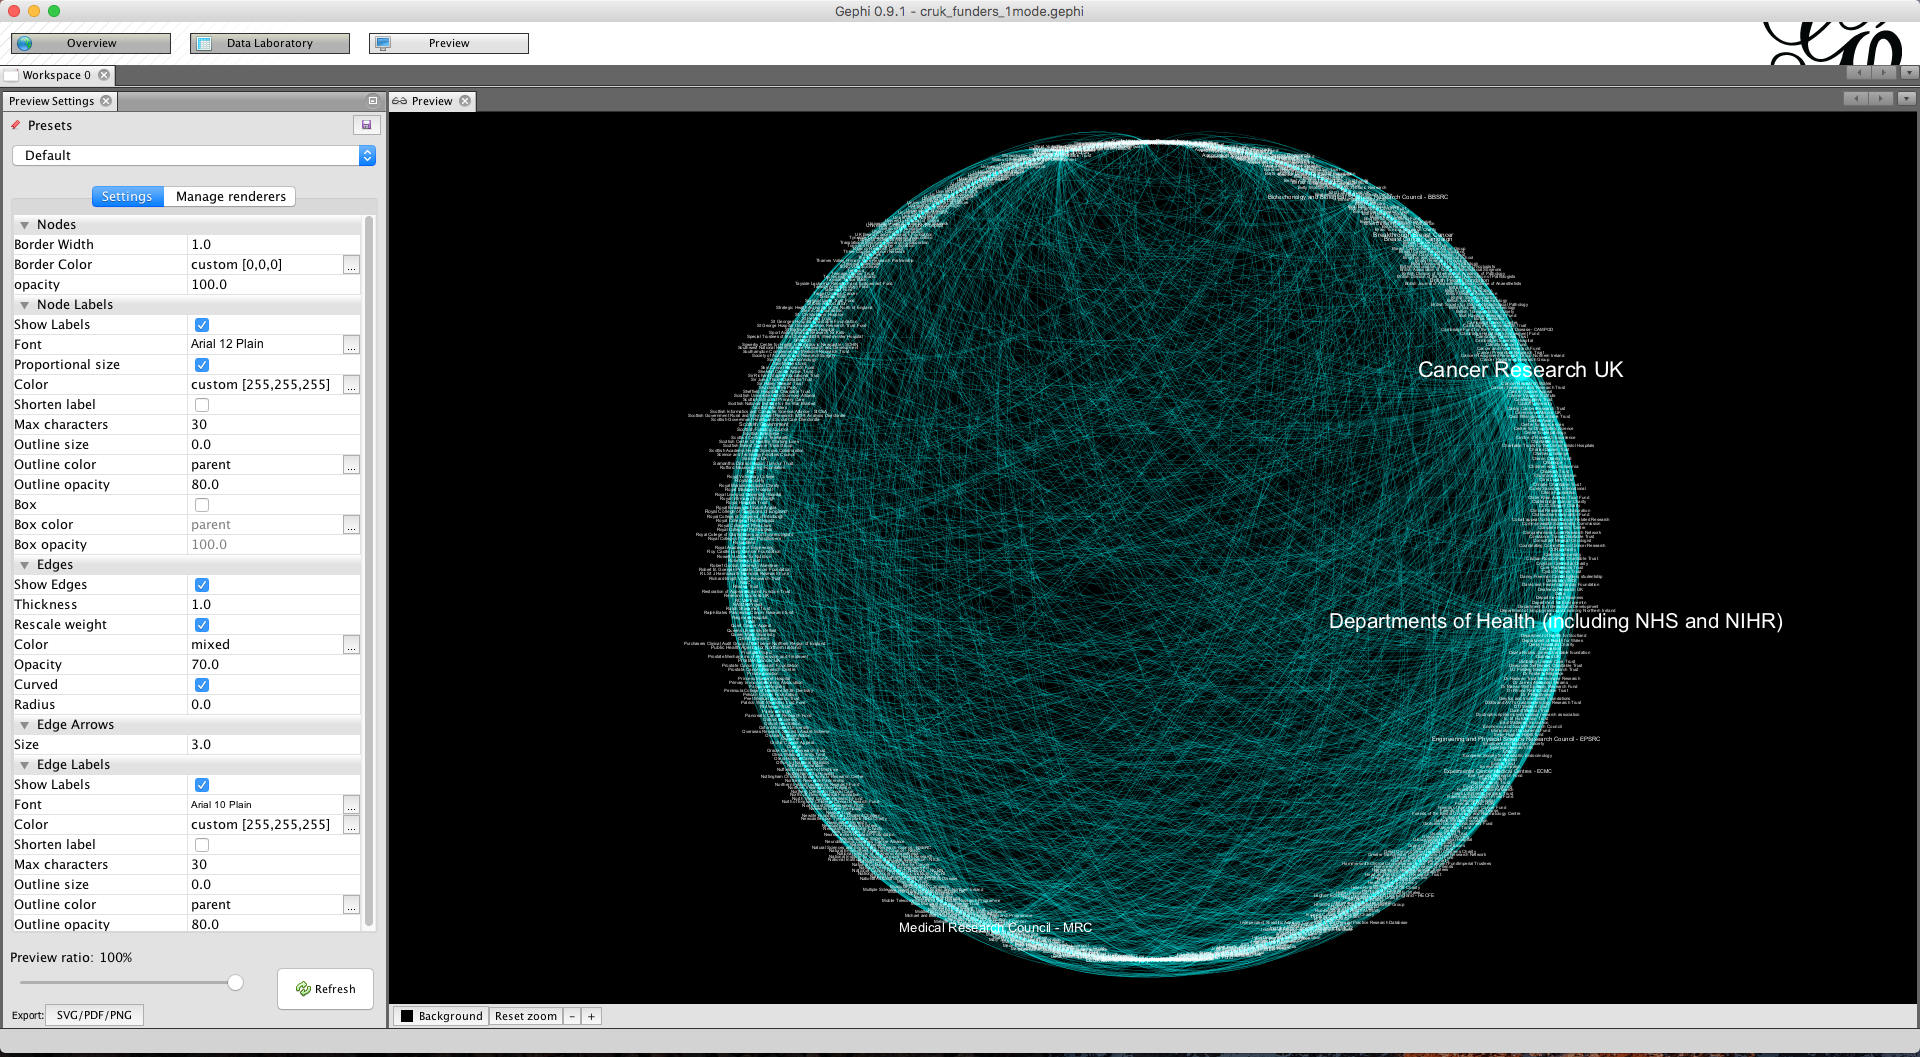
\includegraphics[width=\linewidth, frame]{gephi_interface3}

\end{frame}

%------------------------------------------------

\begin{frame}
\frametitle{\insertsection}
\framesubtitle{Ready?}

\begin{enumerate}
	\item Go to \url{https://gephi.org/}
	\item Download Gephi
	\item Install Gephi* 
\end{enumerate}

\begin{textblock*}{8cm}(0.5cm, 8.5cm)
\scriptsize{*If you are using a computer on campus, install Gephi on your `N' drive}
\end{textblock*}

\end{frame}

%------------------------------------------------

%------------------------------------------------

\begin{frame}
\frametitle{\insertsection}
\framesubtitle{Exercise}

\textbf{Microneedles}: needles the size of which is on the \textit{micrometer} length scale. Expected impact on vaccines, drug delivery, and reduction of biohazard waste
   
\begin{columns}

\column{.45\textwidth}
\begin{minipage}[c][.6\textheight][c]{\linewidth}
\centering
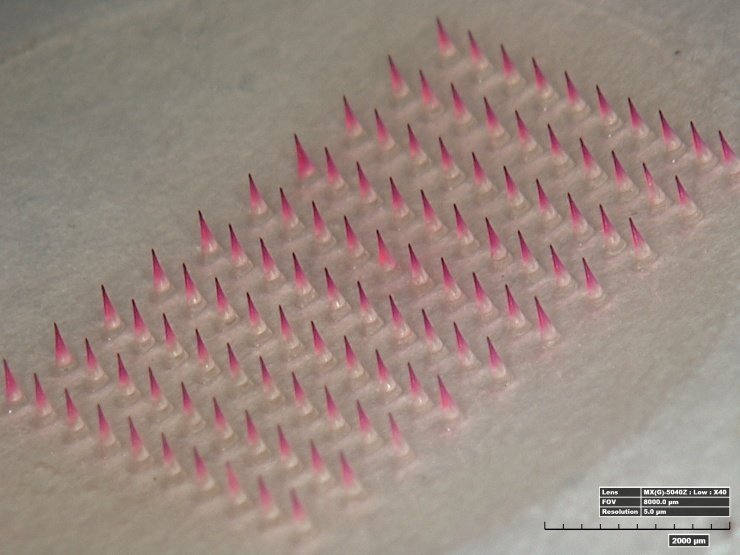
\includegraphics[width=0.8\textwidth,keepaspectratio]{micro1}\\
\tiny{Source: \url{www.news.gatech.edu}}	 	
\end{minipage}
        
\column{.45\textwidth}
\begin{minipage}[c][.6\textheight][c]{\linewidth}
\centering
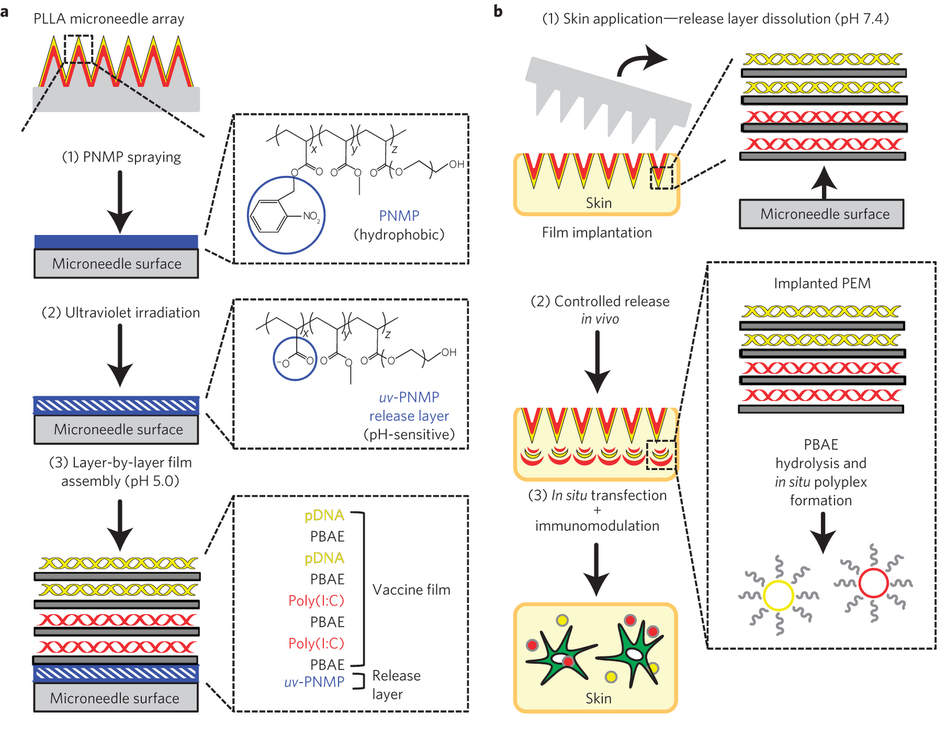
\includegraphics[width=0.8\textwidth,keepaspectratio]{micro2}\\
\tiny{Source: DeMuth PC et al. (2013). Polymer multilayer tattooing for enhanced DNA vaccination. Nature Materials, 12(4), 367-276}
\end{minipage}

\end{columns}


\end{frame}

%------------------------------------------------

\begin{frame}
\frametitle{\insertsection}
\framesubtitle{Exercise}

Objectives of the analysis
\begin{itemize}
	\item To map collaboration activity
	\item To characterise the inter-organisational network
	\item To identify key organisations in this network
\end{itemize}

\end{frame}

%------------------------------------------------

\begin{frame}
\frametitle{\insertsection}
\framesubtitle{Exercise}
   
\textbf{1. Data collection}
    \begin{itemize}          
     \item Search for expert-defined {\color{teal}{keywords}} in publication titles and abstracts
         \begin{itemize}  
         \item \textit{microneedle*} 
         \item \textit{micro-needle*} 
         \item \textit{microprojection patch*} 
         \item \textit{micro-projection patch*}
         \item ...
         \end{itemize}
         		                      
    \item 1,090 publications in the 2010-2014 period
     
    \item 887 organizations (disambiguation of names) 
                   
     \item Classification of the {\color{teal}{organisations by type}}
       		\begin{itemize}
       		\item Research and Higher Education (RHE)
       		\item Healthcare Provider (HCP)
        	\item Government (GOV)
            \item Research Institute (RIN)
            \item Industry (IND)
            \item Non-Government Organization (NGO)
			\end{itemize}
				   
      \item {\color{red}{Assumption:}} Co-authorship = Collaboration (!)
                             
        \end{itemize}

\end{frame}
%------------------------------------------------

\begin{frame}
\frametitle{\insertsection}
\framesubtitle{Exercise}

\begin{columns}
\column{.5\textwidth}

\textbf{2. Data preparation}
\begin{itemize}
	\item Data were pre-processed 
	\item Gephi can import {\color{teal}{Excel files}}
	\item We need to create two files or sheets
	\begin{itemize}
		\item {\color{teal}{Nodes}} table
		\item {\color{teal}{Edges}} table
	\end{itemize}
	\item Format these `tables' as in the file  \textit{``microneedles\_2010\_14\_for\_gephi.xlsx''}
\end{itemize}


\column{.5\textwidth}
\footnotesize
\centering
{\color{teal}{Nodes table}}\\ 
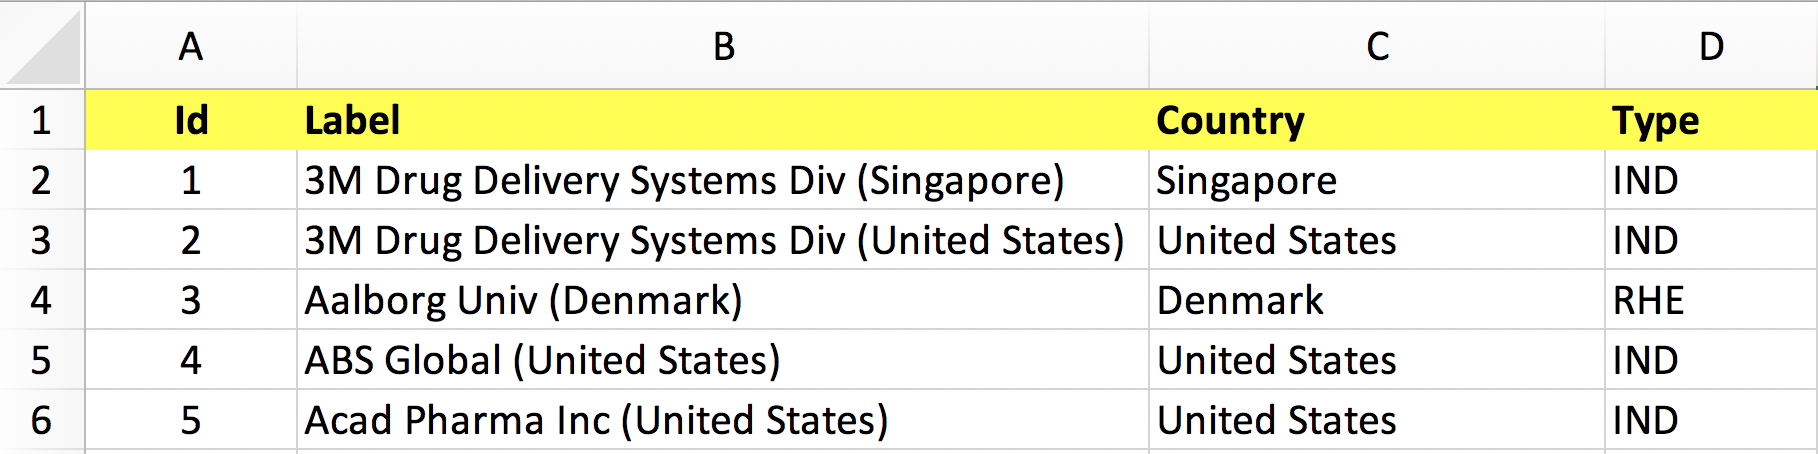
\includegraphics[height = 1.5cm]{gephi_nodes}\\

\medskip
\medskip

{\color{teal}{Edges table}}\\
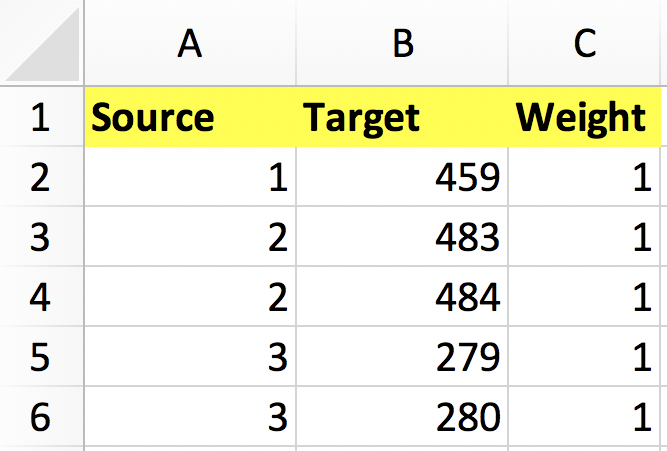
\includegraphics[height = 1.5cm]{gephi_edges}\\

\end{columns}

\end{frame}

%------------------------------------------------

\begin{frame}
\frametitle{\insertsection}
\framesubtitle{Exercise}


\begin{columns}
\column{.5\textwidth}

\textbf{3.Import data into Gephi}
\begin{enumerate}
	\item Create a new project in Gephi
	\item Select \textit{Data Laboratory}
	\item Select \textit{Import Spreadsheet}
		  \begin{itemize}
		  \item 	We first import nodes, then edges
		  \item Remember to import the network as undirected
		  \item Make sure you tick the \textit{Append to existing workspace} option
		  \end{itemize}
	\item Save the project
\end{enumerate}


\column{.5\textwidth}
\footnotesize
\centering
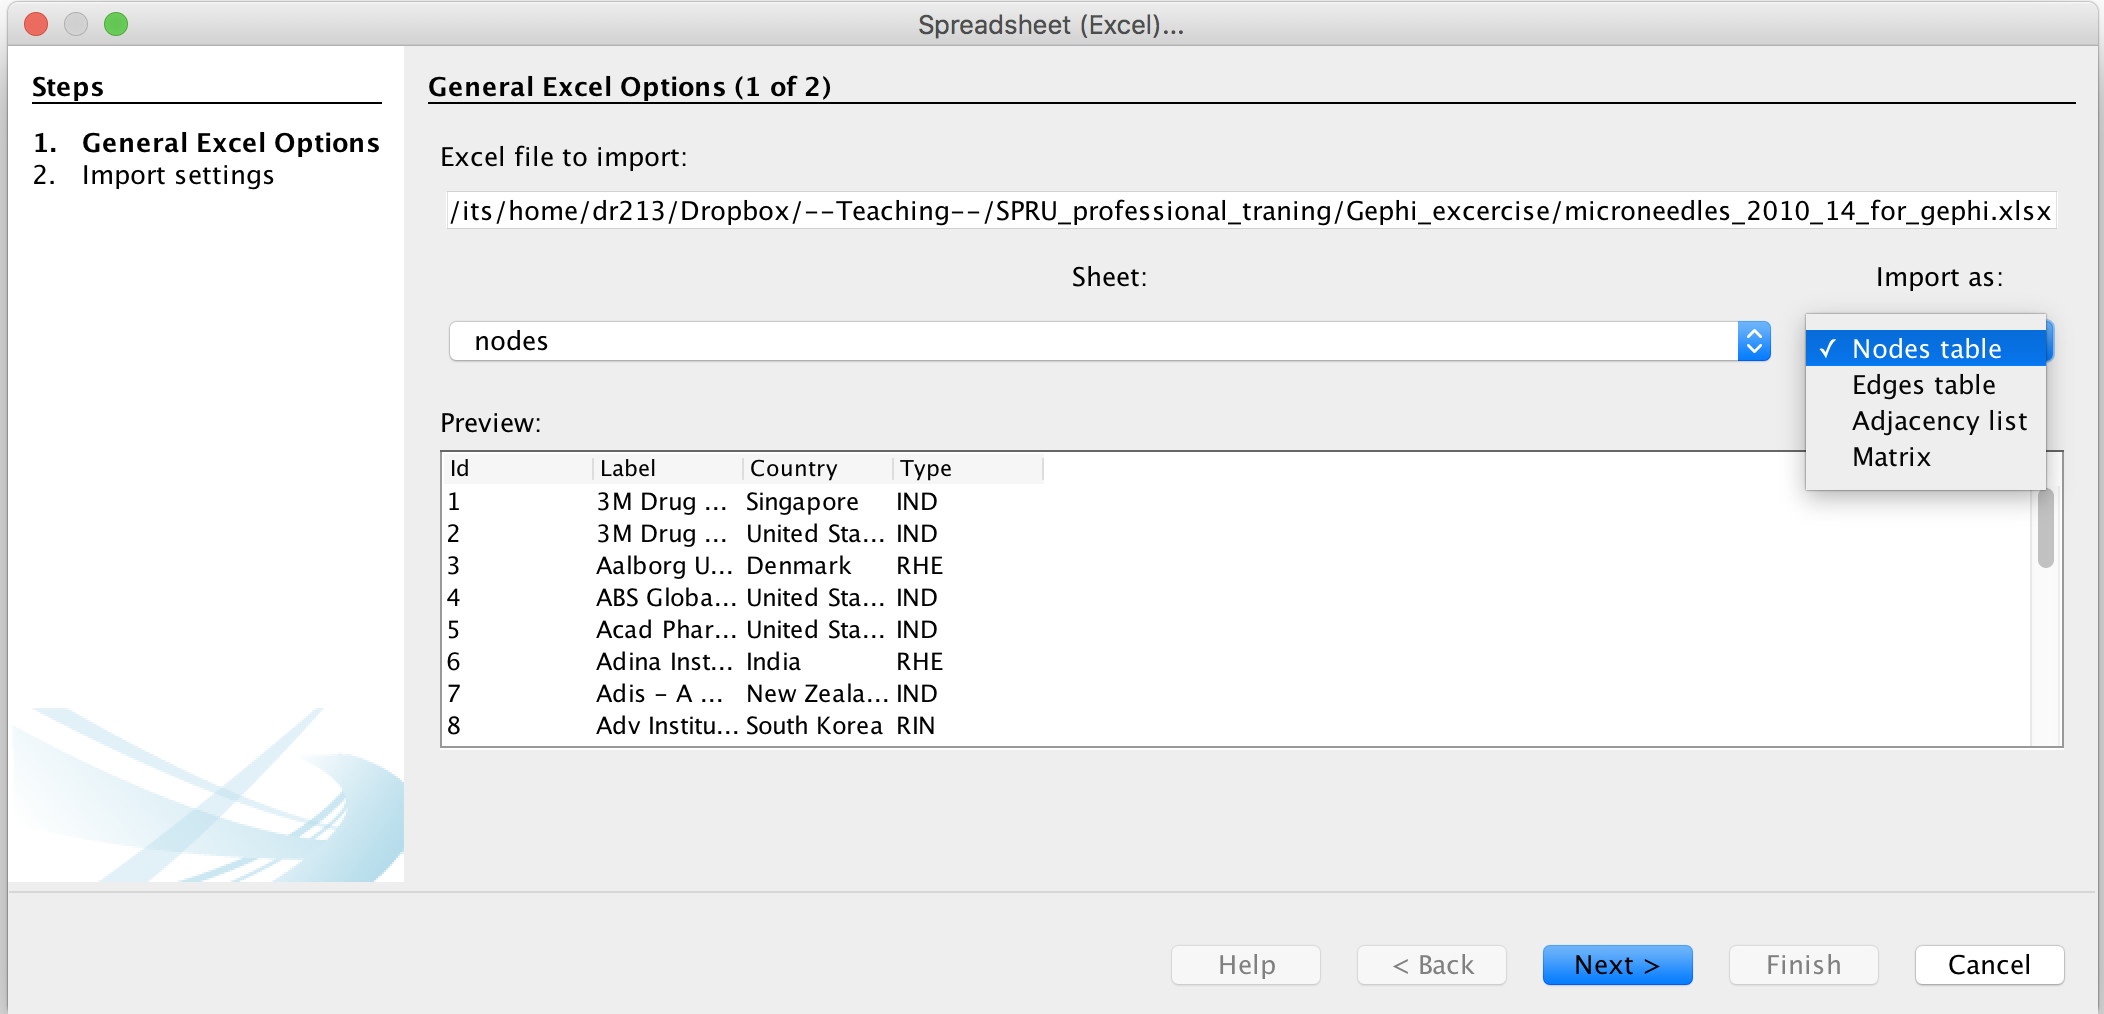
\includegraphics[height = 2.5cm]{nodes_import.png}\\

\medskip
\medskip

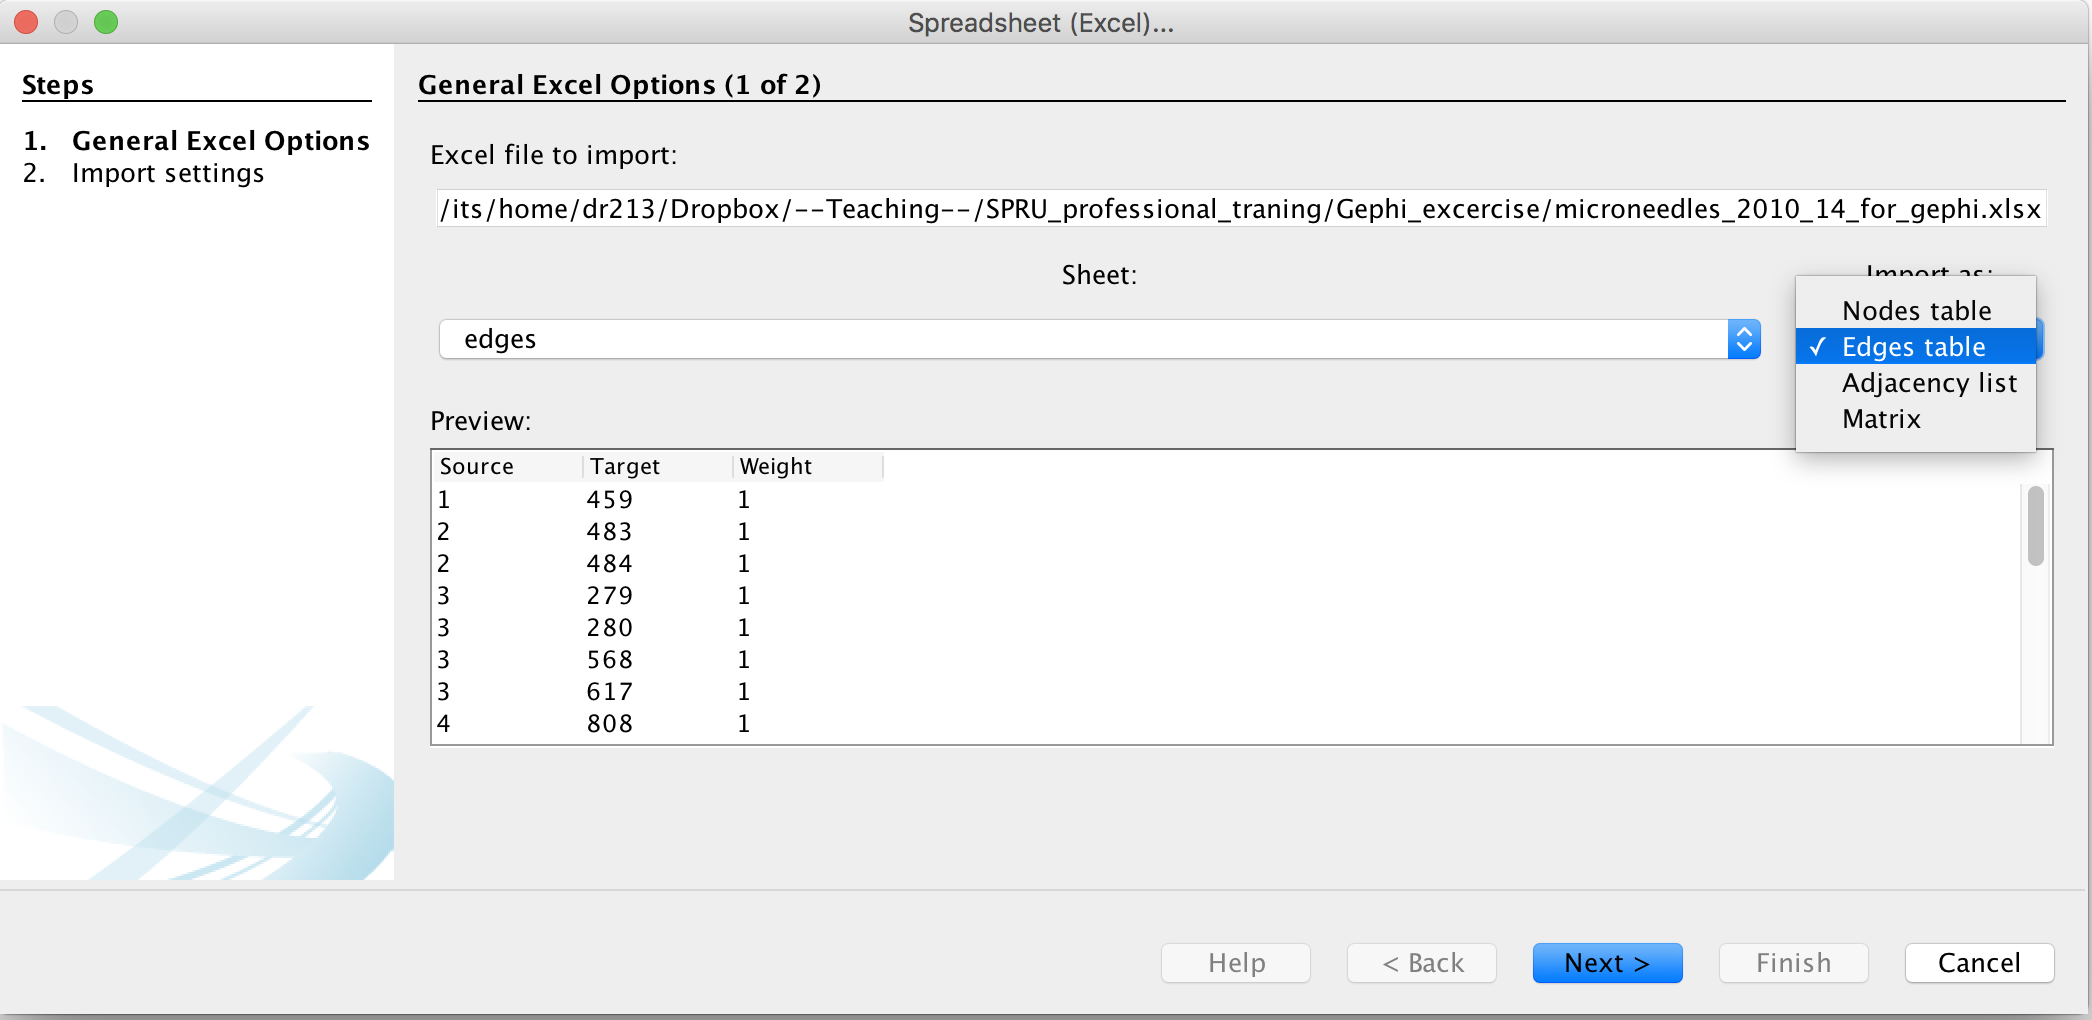
\includegraphics[height = 2.5cm]{edges_import.png}\\


\end{columns}

\end{frame}

%------------------------------------------------

\begin{frame}
\frametitle{\insertsection}
\framesubtitle{Exercise}

\begin{columns}
\column{.5\textwidth}

\textbf{4.Improve the visualisation}
\begin{itemize}
	
\item Colour nodes by type
\begin{enumerate}
	\item Go to \textit{Appearance} in \textit{Overview}
	\item Select \textit{Nodes}, \textit{Colors}, and \textit{Partition}
	\item Select the attribute \textit{type} and \textit{Apply}
\end{enumerate}

\item Improve the layout
\begin{enumerate}
	\item Go to the \textit{Layout} tab
	\item Select a layout algorithm (\textit{Yifan Hu})
	\item Try different layout algorithms
\end{enumerate}

\item Exclude isolates and small components 
\begin{enumerate}
	\item Go to the \textit{Filters} tab
	\item Expand the folder \textit{Topology}
	\item Drag an drop \textit{Giant Component}\\
		  into \textit{Queries} and \textit{Filter}
\end{enumerate}

\item Increase node size by degree
\begin{enumerate}
	\item Go to \textit{Appearance}
	\item Select \textit{Nodes}, \textit{Size}, and \textit{Ranking}
	\item Select the \textit{Degree} attribute 
		 (range from 10 to 50) and \textit{Apply}
\end{enumerate}

\end{itemize}

\column{.5\textwidth}
\footnotesize
\centering
\only<1>{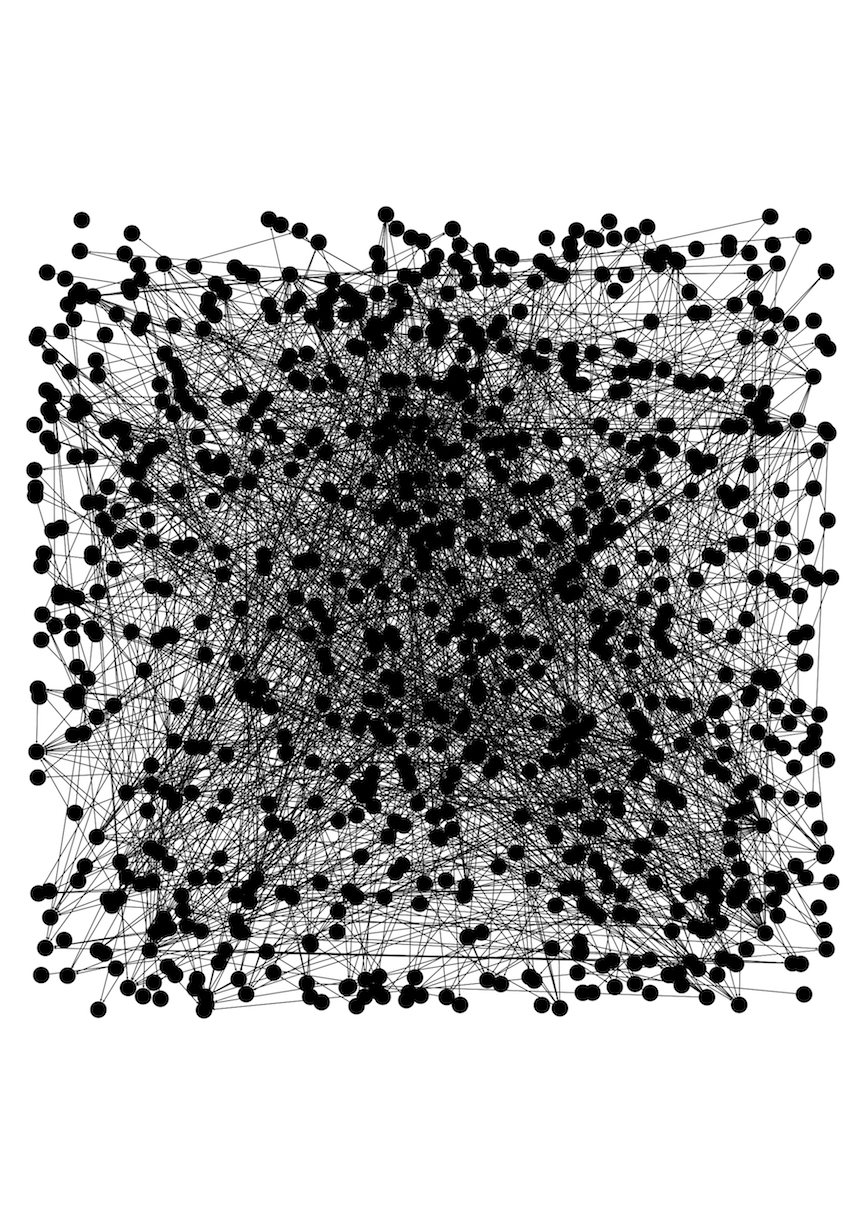
\includegraphics[height = 1.3\textwidth]{step1.jpg}}

\only<2>{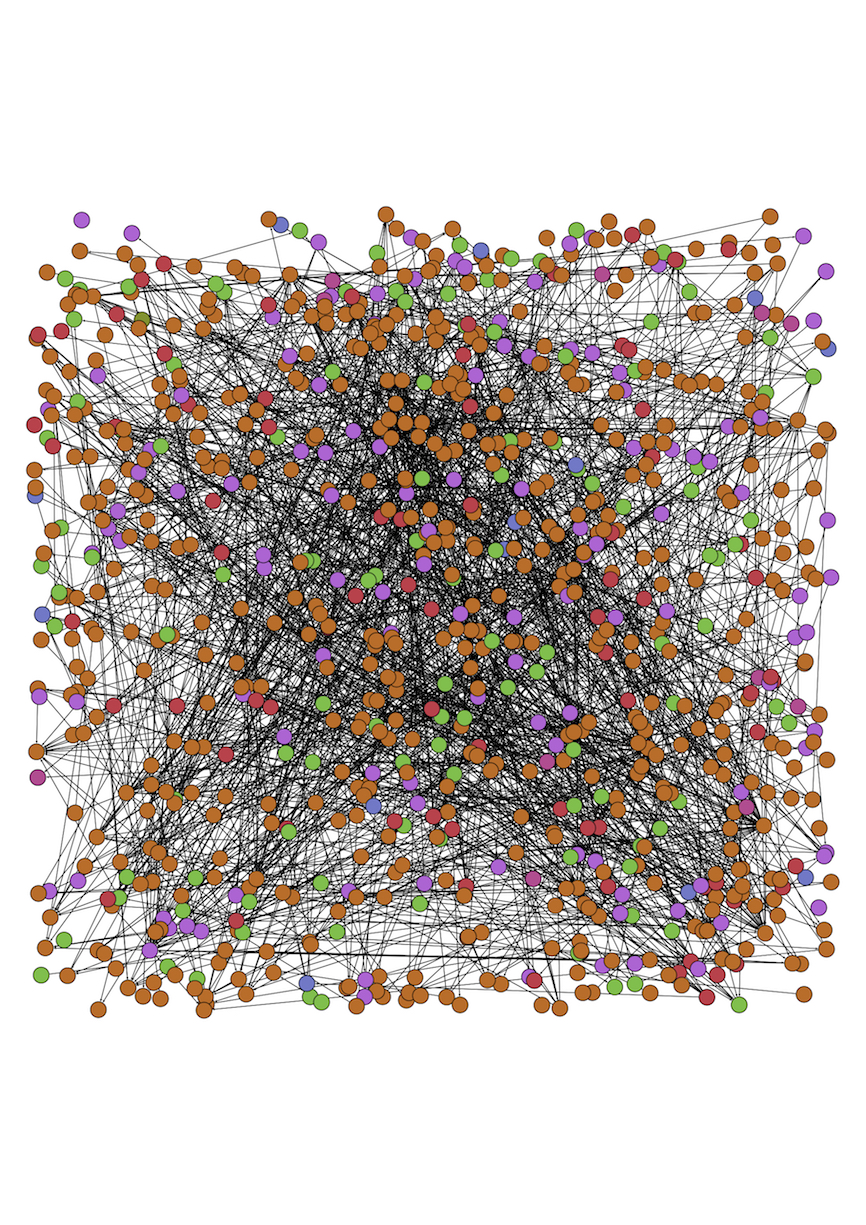
\includegraphics[height = 1.3\textwidth]{step2.jpg}}

\only<3>{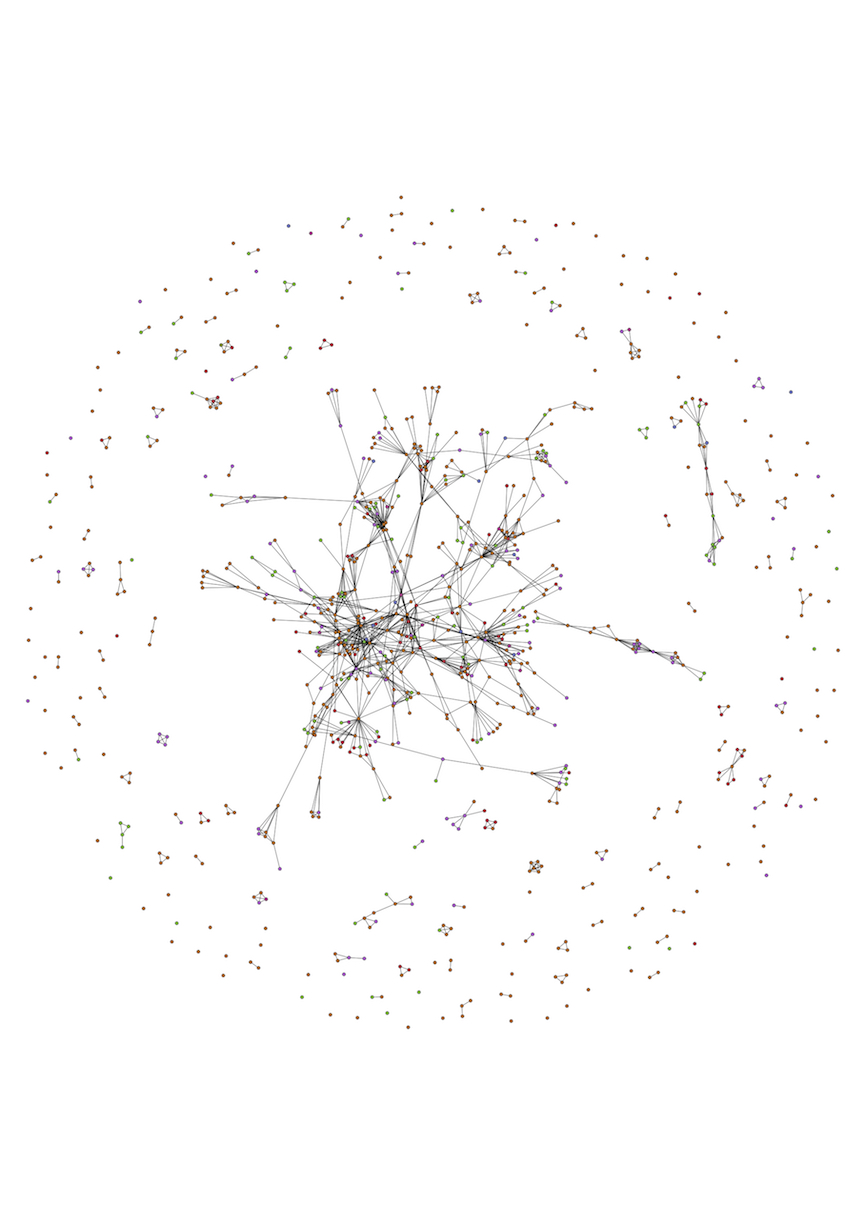
\includegraphics[height = 1.3\textwidth]{step3.jpg}}

\only<4>{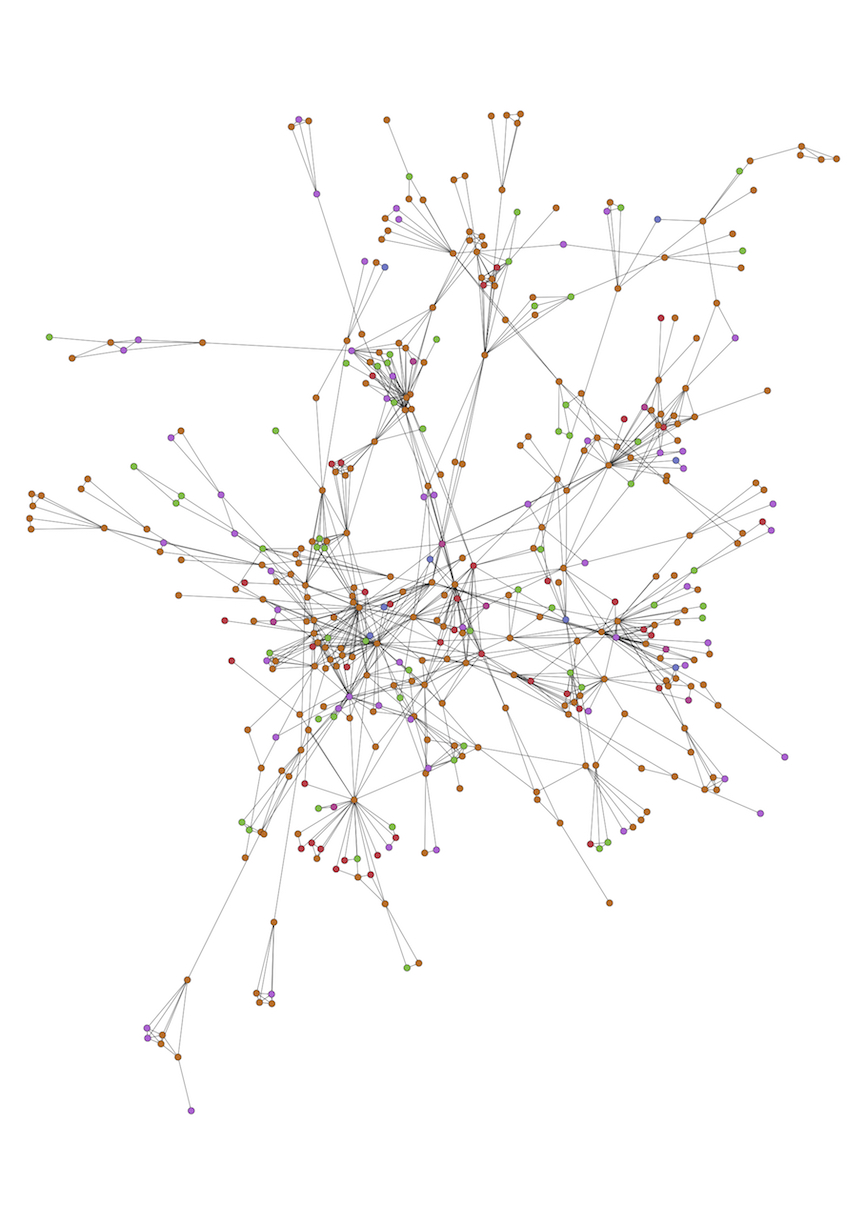
\includegraphics[height = 1.3\textwidth]{step4.jpg}}

\only<5>{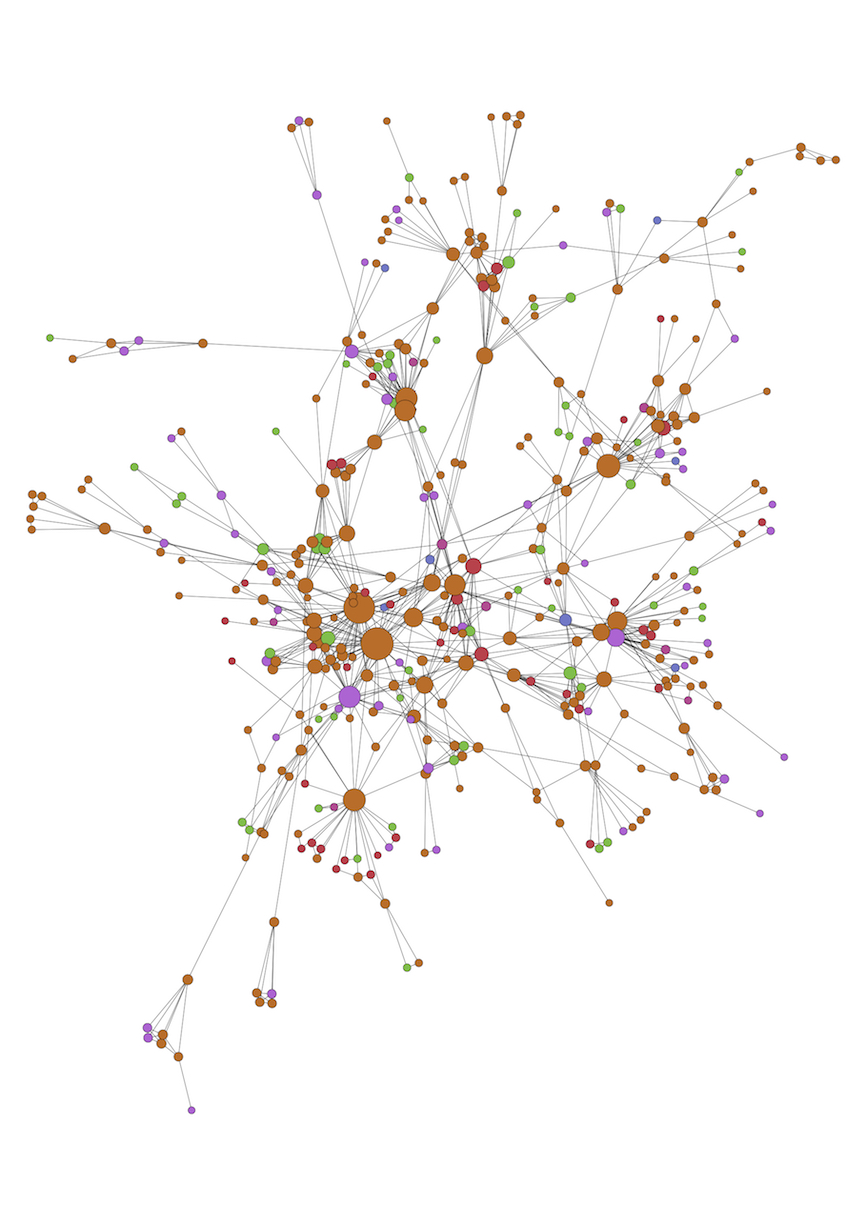
\includegraphics[height = 1.3\textwidth]{step5.jpg}}

\end{columns}

\end{frame}

%------------------------------------------------

\begin{frame}
\frametitle{\insertsection}
\framesubtitle{Exercise}

\begin{columns}
\column{.5\textwidth}

\textbf{5.Characterise the network}
\begin{enumerate}
	\item We can calculate the density  
	\item Go to \textit{Statistics}
	\item Run \textit{Graph Density}
	\item Giant component's density = 0.011
	\item Other measures: Diameter, Components, Modularity, etc.
\end{enumerate}


\column{.5\textwidth}
\footnotesize
\centering
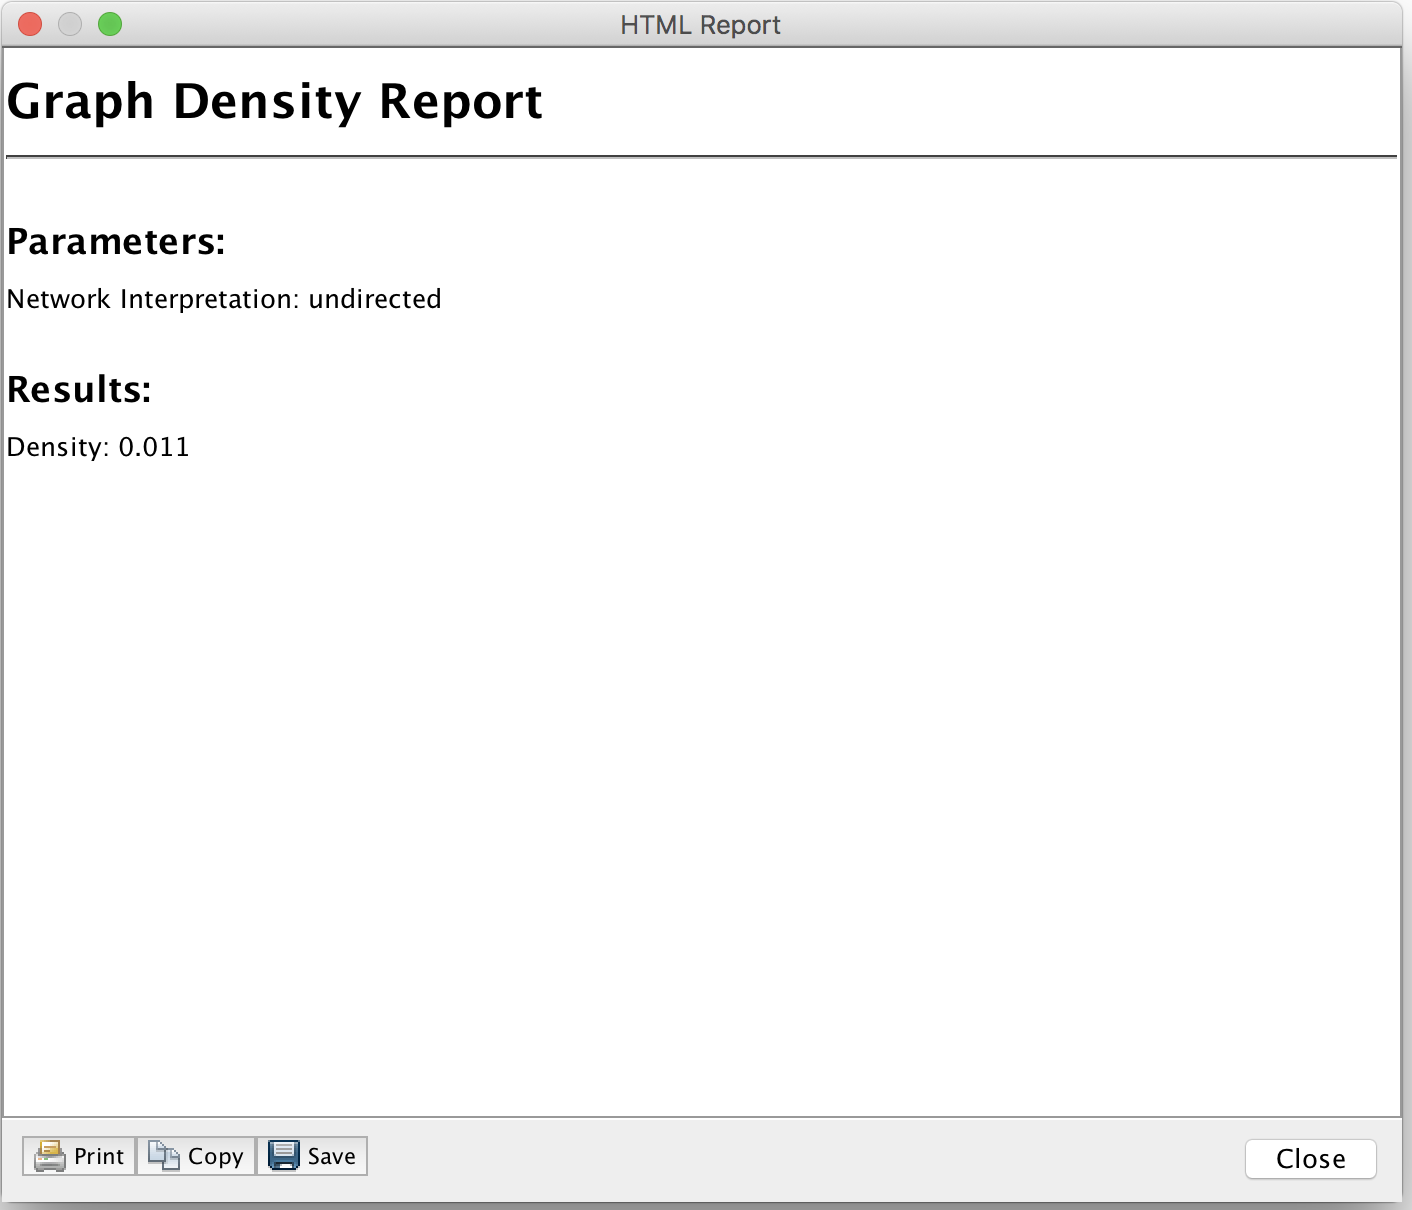
\includegraphics[height = 0.7\textwidth]{gephi_density.png}

\end{columns}

\end{frame}

%------------------------------------------------

\begin{frame}
\frametitle{\insertsection}
\framesubtitle{Exercise}

\textbf{6.Identify key organisations}
\begin{enumerate}
	\item We can calculate centrality measures  
	\item Run \textit{Average Degree}
	\item Run \textit{Network Diameter}\\
	\item Closeness and betweenness are added as attributes (see \textit{Data Laboratory})
\end{enumerate}

\medskip
\medskip

\only<1>{
\scriptsize
\centering
\begin{table}[]
\begin{tabular}{lp{1cm}}
\hline
Organisation                                          & Degree \\
\hline
Georgia Inst of Tech (United States)                  & 41\\
Emory Univ (United States)                            & 39\\
Univ of Queensland (Australia)                        & 27\\
Yonsei Univ, Seoul (South Korea)                      & 25\\
Korea Adv Inst of Sci and Tech (KAIST) (South Korea)  & 24\\
North Carolina State Univ (United States)             & 24\\
Harvard Univ (United States)                          & 23\\
Univ of North Carolina at Chapel Hill (United States) & 23\\
Queen's Univ, Belfast (United Kingdom)                & 21\\
Massachusetts Inst of Tech (United States)			  & 20\\
...\\
\hline
\end{tabular}
\end{table}}


\only<2>{
\scriptsize
\centering
\begin{table}[]
\begin{tabular}{lp{1cm}}
\hline
Organisation                                         & Closeness \\
\hline
Georgia Inst of Tech (United States)                 & 0.31 \\
Emory Univ (United States)                           & 0.31 \\
Massachusetts Inst of Tech (United States)           & 0.30 \\
Korea Adv Inst of Sci and Tech (KAIST) (South Korea) & 0.29 \\
Harvard Univ (United States)                         & 0.29 \\
Seoul Nat Univ (South Korea)                         & 0.29 \\
Cardiff Univ (United Kingdom)                        & 0.28 \\
Sungkyunkwan Univ (South Korea)                      & 0.28 \\
Kangbuk Samsung Hosp (South Korea)                   & 0.28 \\
Univ of Oxford (United Kingdom)                      & 0.27 \\
...\\
\hline
\end{tabular}
\end{table}}


\only<3>{
\scriptsize
\centering
\begin{table}[]
\begin{tabular}{lp{1cm}}
\hline
Organisation                                         & Betweenness\\
\hline
Georgia Inst of Tech (United States)                 & 19108 \\
Osaka Univ (Japan)                                   & 16665 \\
Emory Univ (United States)                           & 16378 \\
Cardiff Univ (United Kingdom)                        & 14442 \\
Harvard Univ (United States)                         & 13327 \\
Univ of Queensland (Australia)                       & 13072 \\
Massachusetts General Hosp (United States)           & 12001 \\
Korea Adv Inst of Sci and Tech (KAIST) (South Korea) & 11620 \\
Seoul Nat Univ (South Korea)                         & 10648 \\
Massachusetts Inst of Tech (United States)           & 10631 \\
...\\
\hline
\end{tabular}
\end{table}}

\end{frame}

%------------------------------------------------

\begin{frame}
\frametitle{\insertsection}
\framesubtitle{Exercise}

\begin{columns}
\column{.5\textwidth}

\textbf{7.Visualising ego networks}
\begin{enumerate}
    \item We can visualise the ego network of the Georgia Inst of Tech
	\item Go to \textit{Filters}
	\item Expand the folder \textit{Topology}
	\item Drag an drop \textit{Ego Network}\\
		  into \textit{Queries}
	\item Select \textit{Node Id} and \textit{Filter}
\end{enumerate}


\column{.5\textwidth}
\footnotesize
\centering
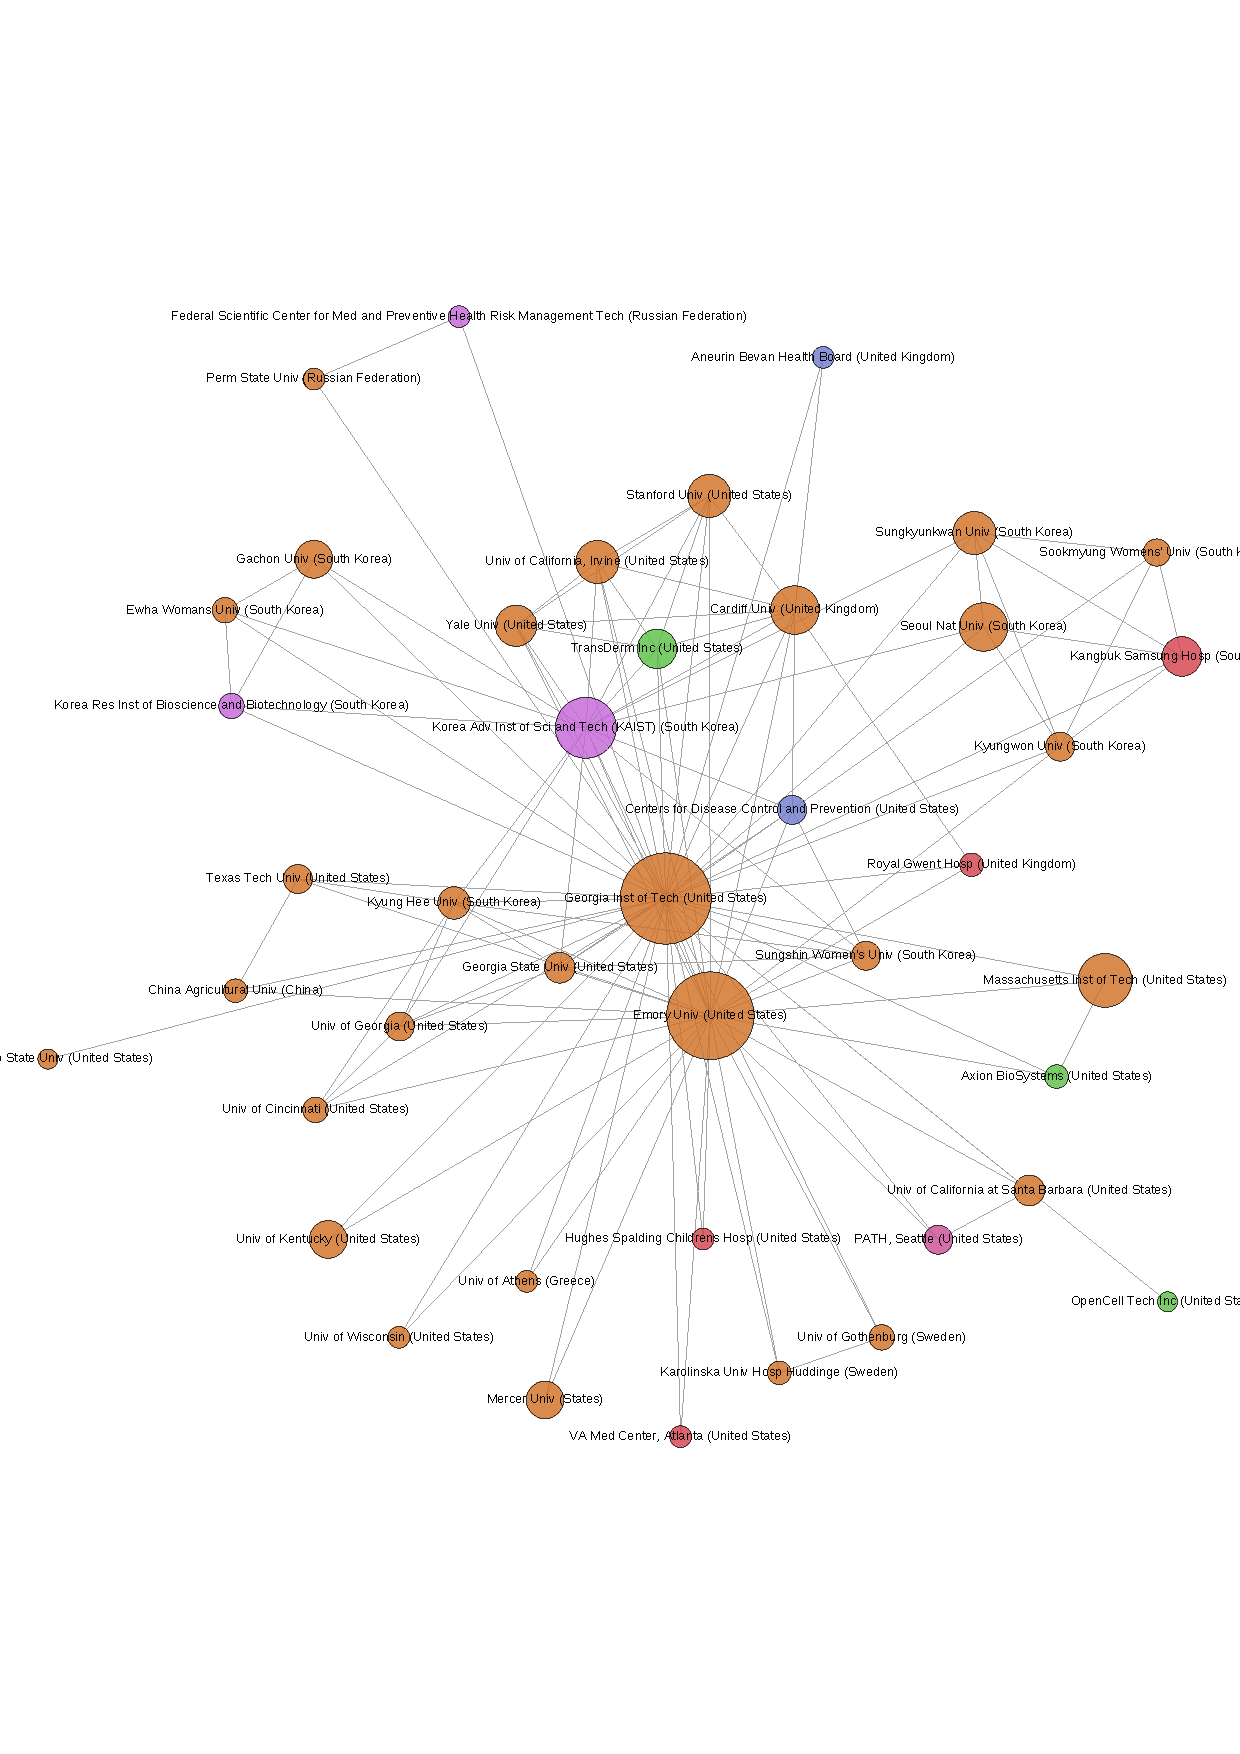
\includegraphics[height = 1.3\textwidth]{gephi_ego}

\end{columns}

\end{frame}

%------------------------------------------------




%%=======================================================
%	Next time ...
%%=======================================================
\section*{Next time ...}
%------------------------------------------------

\bgroup
\setbeamercolor{background canvas}{bg = navyblue}
\begin{frame}[plain]{}
\begin{center}
\color{white}{\Huge\insertsection}
\end{center}
\end{frame}
\egroup

%------------------------------------------------

\begin{frame}
\frametitle{\insertsection}

\begin{itemize}

\item 	\textbf{Lecture: Network models}
	\begin{itemize}
	\item Mathematical models of network analysis
	\item Overview of statistical models of network analysis
	\end{itemize}	


\medskip
\medskip


\item 	\textbf{Seminar: Network models}
	\begin{itemize}
	\item Network mathematical models in igraph
	\item Gephi exercise
	\end{itemize}
	
\end{itemize}

\end{frame}

%------------------------------------------------






\end{document}